% arara: pdflatex: { options: ["--synctex=1", "-interaction=nonstopmode"] }
% arara: bibtex
% arara: pdflatex: { options: ['-synctex=1', '-interaction=nonstopmode'] }
% arara: pdflatex: { options: ['-synctex=1', '-interaction=nonstopmode'] }
%%
%% Copyright 2022 OXFORD UNIVERSITY PRESS
%%
%% This file is part of the 'oup-authoring-template Bundle'.
%% ---------------------------------------------
%%
%% It may be distributed under the conditions of the LaTeX Project Public
%% License, either version 1.2 of this license or (at your option) any
%% later version.  The latest version of this license is in
%%    http://www.latex-project.org/lppl.txt
%% and version 1.2 or later is part of all distributions of LaTeX
%% version 1999/12/01 or later.
%%
%% The list of all files belonging to the 'oup-authoring-template Bundle' is
%% given in the file `manifest.txt'.
%%
%% Template article for OXFORD UNIVERSITY PRESS's document class `oup-authoring-template'
%% with bibliographic references
%%

%%%CONTEMPORARY%%%
%\documentclass[unnumsec,webpdf,contemporary,large]{oup-authoring-template}%
%\documentclass[numsec,webpdf,modern,large]{oup-authoring-template}% uncomment this line for author year citations and comment the above
%\documentclass[unnumsec,webpdf,contemporary,medium]{oup-authoring-template}
%\documentclass[unnumsec,webpdf,contemporary,small]{oup-authoring-template}

%%%MODERN%%%
%\documentclass[unnumsec,webpdf,modern,large]{oup-authoring-template}
\documentclass[unnumsec,webpdf,modern,large,namedate]{oup-authoring-template}% uncomment this line for author year citations and comment the above
%\documentclass[unnumsec,webpdf,modern,medium]{oup-authoring-template}
%\documentclass[unnumsec,webpdf,modern,small]{oup-authoring-template}

%%%TRADITIONAL%%%
%\documentclass[unnumsec,webpdf,traditional,large]{oup-authoring-template}
%\documentclass[unnumsec,webpdf,traditional,large,namedate]{oup-authoring-template}% uncomment this line for author year citations and comment the above
%\documentclass[unnumsec,namedate,webpdf,traditional,medium]{oup-authoring-template}
%\documentclass[namedate,webpdf,traditional,small]{oup-authoring-template}

%\onecolumn % for one column layouts

%\usepackage{showframe}

\graphicspath{{Fig/}}

% --- packages you added ---
\usepackage{booktabs}
\usepackage{amsmath, amssymb}
\usepackage{subfig}
\usepackage{hyperref}
\usepackage{cleveref}

% --- theorem styles already defined in your file ---
\theoremstyle{thmstyleone}\newtheorem{theorem}{Theorem}
\newtheorem{proposition}[theorem]{Proposition}
\theoremstyle{thmstyletwo}\newtheorem{example}{Example}
\newtheorem{remark}{Remark}
\theoremstyle{thmstylethree}\newtheorem{definition}{Definition}

\begin{document}

\journaltitle{Bioinformatics}
\DOI{DOI HERE}
\copyrightyear{2025}
\pubyear{2025}
\access{Advance Access Publication Date: Day Month Year}
\appnotes{Original Paper}

\firstpage{1}

\title[Tensor Co-clustering for C. elegans Morphogenesis]{Discovering Coordinated Cell Behavior in \textit{C.~elegans} Morphogenesis with Tensor Co-clustering}

\author[1,$\ast$]{Zihan Wu}
\author[1]{Zhaoke Huang}
\author[1]{Zelin Li}
\author[1]{Hong Yan}

\authormark{Wu et al.}

\address[1]{\orgdiv{Department of Electrical Engineering}, \orgname{City University of Hong Kong}, \orgaddress{\country{Hong Kong SAR, China}}}

\corresp[$\ast$]{Corresponding author. \href{mailto:wzh4464@gmail.com}{wzh4464@gmail.com}}

\received{Date}{0}{Year}
\revised{Date}{0}{Year}
\accepted{Date}{0}{Year}

\abstract{
\textbf{Motivation:} The embryonic development of the nematode \textit{Caenorhabditis elegans} is captured by modern 4D microscopy, yielding rich spatio-temporal datasets. Automatically discovering groups of cells that behave coordinately over particular time windows remains challenging when matrix-based representations disrupt higher-order relationships.\\
\textbf{Results:} We introduce DiMergeTCC, a tensor co-clustering framework that extends Distributed Merge Co-clustering from matrices to tensors (cells $\times$ time $\times$ features), preserving probabilistic guarantees while scaling to large 4D datasets. Applied to an embryonic dataset, DiMergeTCC unbiasedly recovered two hallmark morphogenetic events: dorsal intercalation of dorsal epithelium and the organization/polarization of the intestinal primordium.\\
\textbf{Availability:} Code and reproducible pipelines: \href{https://github.com/your-org/DiMergeTCC}{GitHub (to be released upon publication)}.\\
\textbf{Contact:} \href{mailto:wzh4464@gmail.com}{wzh4464@gmail.com}
}

\keywords{Tensor co-clustering, \textit{C. elegans}, morphogenesis, spatio-temporal data, computational biology}

\maketitle

% ------------------------ INTRODUCTION ------------------------
\section{Introduction}

The process of morphogenesis, by which an organism develops its shape, is driven by a complex symphony of coordinated cellular behaviors, including migration, division, and changes in morphology and adhesion. The nematode Caenorhabditis elegans has long served as a pre-eminent model organism for studying these fundamental processes. Its largely invariant cell lineage, optical transparency, and rapid development allow for the complete tracking of every cell from fertilization to hatching using 4D (3D space + time) light microscopy~\citep{kaletta2006FindingFunctionNovel,hwang2003CaenorhabditisElegansEarly}.

The resulting datasets are a rich resource but present a formidable analytical challenge. They encapsulate the spatio-temporal trajectories and feature dynamics of hundreds of cells over thousands of time points. A key goal in analyzing this data is to move beyond tracking individual cells to identifying functional modules: groups of cells that act in a coordinated manner over specific periods of development. Such collective behaviors are the building blocks of tissue formation and organogenesis~\citep{setty2008FourdimensionalRealisticModeling}.

Traditional computational approaches often simplify this high-dimensional data by "flattening" it into a two-dimensional matrix, for instance, by concatenating time points or features. This process of matricization, however, fundamentally disrupts the inherent multi-way structure of the data. The intricate, higher-order interactions between cells, their dynamic features (e.g., velocity, shape), and time are obscured, limiting the discovery of complex patterns.

Tensors, or multi-dimensional arrays, provide a more natural and powerful framework for representing such data, preserving these relationships~\citep{sun2008IncrementalTensorAnalysis}. A tensor of dimensions (cells × time × features) can holistically capture the system's dynamics. To analyze this representation, we require computational tools capable of identifying meaningful sub-structures within the tensor.

In this work, we propose a novel framework for this purpose by extending the Distributed Merge Co-clustering (DiMergeCo) algorithm from matrices to tensors. Co-clustering, or biclustering, simultaneously groups rows and columns of a matrix, and has proven highly effective in bioinformatics for finding local patterns, such as subsets of genes that are co-expressed under a subset of conditions~\citep{zapala2006MultivariateRegressionAnalysis}. Our tensor extension, DiMergeTCC, identifies "co-clusters" that are cohesive blocks within the data tensor, corresponding to groups of cells exhibiting similar feature dynamics over contiguous time intervals. Critically, our extension maintains the strong probabilistic guarantees of the original DiMergeCo for preserving co-cluster integrity during the analysis of large datasets.

To validate our approach, we applied it to a comprehensive 4D dataset of C. elegans embryogenesis. By analyzing a rich set of features including 3D shape descriptors, kinematics, and lineage information, our method successfully rediscovered two well-characterized morphogenetic events without any a priori biological annotation: dorsal intercalation and the formation of the intestinal primordium~\citep{bao2006AutomatedCellLineage,kaletta1997BinarySpecificationEmbryonic,artal-sanz2006CaenorhabditisElegansVersatile,sato2015LeftRightAsymmetric,stoeckius2009LargescaleSortingElegans}. This demonstrates that DiMergeTCC is a powerful, unbiased tool for pattern discovery in high-dimensional developmental data, capable of generating concrete, biologically meaningful hypotheses.

\section{Background and Related Work}

Our work is situated at the intersection of three domains: the computational analysis of C. elegans morphogenesis, co-clustering algorithms, and tensor-based data mining in biology.

\subsection{Data acquisition and imaging/segmentation pipeline}
We used the CMap platform to obtain \textit{C.~elegans} embryonic 4D imaging and cell-level morphological data. Embryos co-expressed a nuclear marker (HIS-72::GFP) and a membrane marker (mCherry-PH(PLC1$\delta$1)) and were imaged on a Leica SP8 confocal microscope. Each session acquired two channels across \textbf{92 $z$-planes}, with $x/y$ resolution of 0.09~$\mu$m/pixel, $z$-resolution of 0.42~$\mu$m/pixel, and a temporal resolution of $\sim$1.5~min/frame. The full pipeline included deconvolution, automated lineage tracking (StarryNite/AceTree), and membrane segmentation (EDT-DMFNet), producing for each time point: \textbf{cell identity, lineage/fate, shape descriptors, volume ($V$), surface area ($A_S$), and cell--cell contact area ($A_C$)}.

To improve data quality, the raw pipeline incorporates strategies for handling abnormal voxel clusters (e.g., apoptotic ``solid'' fluorescence blobs) and membrane undersampling due to low $z$-resolution. Acquisition parameters were tuned to balance signal intensity and phototoxicity (block scanning, pinhole and laser power compensation). The resulting morphological maps cover $>95\%$ of cells with $<8\%$ missingness.

\subsection{Feature extraction}

\subsubsection{Basic morphological quantities}
From each 3D segmented cell, we compute:
\begin{itemize}
    \item Volume $V$: voxel count $\times$ voxel size.
    \item Surface area $A_S$: alpha-shape triangulation of the membrane surface.
    \item Contact area $A_C$: total area of membrane--membrane interfaces with neighbors.
\end{itemize}
We further define a \textbf{dimensionless irregularity index}
\[
\eta = \frac{\sqrt{A_S}}{\sqrt[4]{V^3}},
\]
which measures deviation from a sphere and captures deformation intensity during migration/intercalation.

\subsubsection{3DCSQ shape spectral features}
To obtain compact and comparable shape descriptors, we follow the \textbf{3DCSQ} approach: each membrane surface is parameterized to the sphere and expanded in spherical harmonics, followed by PCA to extract three types of vectors:
\begin{enumerate}
    \item \textit{eigengrid}$_k$: principal components of the spherical mesh weights.
    \item \textit{eigenharmonic}$_k$: principal components of spherical harmonic coefficients.
    \item \textit{eigenspectrum}$_\ell$: power spectrum coefficients of the harmonics.
\end{enumerate}
These features preserve local detail while enabling reconstruction; we distinguish \textbf{static} features $f_{\text{static}}$ (per-frame) and \textbf{dynamic} features $f_{\text{dynamic}}$ (average over a cell's lifetime).  
For interpretability, we retain components in descending order of explained variance until a target reconstruction error is met.

\subsubsection{Temporal and lineage alignment}
We align each embryo's timeline so that the end of the 4-cell stage is $t=0$. All datasets are resampled to a common frame rate (1.5~min) by linear interpolation; lineage mappings follow CMap's identity files. Missing frames are filled by nearest-neighbor interpolation and masked to avoid artificial correlations in co-clustering.

\subsection{Feature dictionary}
Table~\ref{tab:feature-dict} lists the features used to build the tensor. Morphological derivatives ($\Delta$) are computed as frame-to-frame differences.

\begin{table*}[t]
\centering
\caption{Feature dictionary for tensor construction.}
\label{tab:feature-dict}
\begin{tabular}{llp{9cm}}
\toprule
\textbf{Category} & \textbf{Name} & \textbf{Description} \\
\midrule
Morphology & $V$ & Volume (voxel count $\times$ voxel size) \\
 & $A_S$ & Surface area from alpha-shape triangulation \\
 & $A_C$ & Total membrane--membrane contact area with neighbors \\
 & $\eta$ & Irregularity index: $\sqrt{A_S}/\sqrt[4]{V^3}$ \\
 & $\Delta V$, $\Delta A_S$, $\Delta A_C$ & First-order temporal derivatives of $V$, $A_S$, $A_C$ \\
\midrule
3DCSQ (static) & eigengrid$_{1\ldots K_g}$ & PC scores from spherical mesh vertex positions \\
 & eigenharmonic$_{1\ldots K_h}$ & PC scores from spherical harmonic coefficients \\
 & eigenspectrum$_{0\ldots L_s}$ & Power spectrum coefficients of spherical harmonics \\
\midrule
3DCSQ (dynamic) & dyn\_eigengrid$_{1\ldots K_g}$ & Lifetime-averaged eigengrid components \\
 & dyn\_eigenharmonic$_{1\ldots K_h}$ & Lifetime-averaged eigenharmonic components \\
 & dyn\_eigenspectrum$_{0\ldots L_s}$ & Lifetime-averaged eigenspectrum coefficients \\
\bottomrule
\end{tabular}
\end{table*}

In practice, we set $K_g = 15$, $K_h = 15$, and $L_s = 20$ based on variance explained ($\geq 95\%$) and reconstruction error $<5\%$.

\subsection{Tensor construction}
For each cell $c = 1,\dots,C$ and time $t = 1,\dots,T$, we concatenate all standardized features (z-score using training-set mean/variance) to form $\mathbf{z}_{c,t} \in \mathbb{R}^F$. Stacking over cells and time yields a third-order tensor:
\[
\mathcal{X} \in \mathbb{R}^{C \times T \times F}, \quad \mathcal{X}(c,t,f) = z_{c,t}^{(f)}.
\]
The feature set includes all items in Table~\ref{tab:feature-dict}.

\subsection{Tensor Co-Clustering (TCC): Extending DiMergeCo to three modes}

\subsubsection{Objective and model}
We extend the \textbf{Distributed Merge Co-clustering} (DiMergeCo) framework from matrices to tensors to jointly discover \textbf{cell subsets $\times$ time windows $\times$ feature subsets}. We adopt a tensor block model: within each block $(\mathcal{I}_u,\mathcal{J}_u,\mathcal{K}_u)$, the entries are well-approximated by a low-rank or block-constant structure:
\[
\min_{\{\mathcal{I}_u,\mathcal{J}_u,\mathcal{K}_u\}}
\sum_{u=1}^{U} \left\| \mathcal{X}_{\mathcal{I}_u,\mathcal{J}_u,\mathcal{K}_u} - \hat{\mathcal{X}}_u \right\|_F^2
\]
subject to $\hat{\mathcal{X}}_u$ being low-rank/block-constant.

\subsubsection{Probabilistic partitioning in three modes}
Following DiMergeCo's ``probability of preservation'' principle, we stochastically generate:
\begin{itemize}
    \item \textbf{Cell-mode candidates}: weighted by lineage/space proximity and activity ($\eta$, derivatives), to avoid splitting correlated cells.
    \item \textbf{Time-mode candidates}: multi-scale sliding windows ($16$, $32$, $64$ frames) to capture both short cell-cycle changes and longer organogenesis events.
    \item \textbf{Feature-mode candidates}: initialized by mutual information and correlation thresholds (morphology and 3DCSQ features mixed in layers), with collinear components sparsified.
\end{itemize}
By repeating the partitioning $T_p$ times, true blocks of size above a minimum threshold are likely ($\geq 1-\delta$) to appear intact in at least one candidate, reducing fragmentation risk.

\subsubsection{Local three-way clustering (parallel)}
For each candidate $(\mathcal{I},\mathcal{J},\mathcal{K})$:
\begin{enumerate}
    \item \textbf{Mode-3 unfolding + biclustering}: unfold along features to a $(\mathcal{I} \times \mathcal{J}) \times \mathcal{K}$ matrix and perform simultaneous cell--time biclustering (e.g., SCC or PNMTF).
    \item \textbf{Feature regrouping}: given cell--time sub-blocks, cluster features by within-block variance contribution or loading magnitude.
    \item \textbf{Low-rank estimation}: apply rank-1 or small-rank Tucker approximation to score each block (density, lift, variance explained).
\end{enumerate}
This stage is fully parallelizable; each worker processes distinct blocks.

\subsubsection{Hierarchical merging and deduplication}
All local blocks are inserted into a priority queue sorted by composite score. Blocks with high \textbf{three-mode Jaccard} overlap and non-decreasing score upon merging are merged (three-mode union) until convergence.

\subsection{Statistical assessment and robustness}
\begin{itemize}
    \item \textbf{Permutation/shift tests}: circularly shift time mode and shuffle features within groups to estimate empirical null distributions; control FDR by Benjamini--Hochberg.
    \item \textbf{Individual consistency}: leave-one-embryo-out validation; report weighted Jaccard similarity across embryos.
    \item \textbf{Missing-data sensitivity}: inject 5--20\% extra missingness on top of the real mask and measure recovery rate and score variation.
\end{itemize}

\subsection{Implementation and reproducibility}
Morphological/contact quantities and $\eta$ follow CMap's definitions; 3DCSQ features use the authors' public implementation (SPHARM+PCA), both static and dynamic versions are available. Our tensor is built primarily from per-frame static features; dynamic features are used in post hoc interpretation. All code is in Python/Rust with MPI-based parallelization; seeds are fixed. Preprocessing scripts, feature lists, and hyperparameters are provided in Supplementary Materials.

% ------------------------ RESULTS ------------------------
\section{Biological Validation on \textit{C.~elegans} Embryogenesis}
\label{sec:celegans_validation}

\subsection{Validation design and pre-registered behavioral criteria}
To evaluate whether our tensor co-clustering framework (Sec.~\ref{sec:methods}) recovers \emph{established} morphogenetic behaviors in \textit{C.~elegans}, we designed a literature-grounded validation that operationalizes two canonical processes with well-defined spatiotemporal signatures: (i) \textbf{dorsal intercalation} of hypodermal (hyp) cells (convergent extension across the dorsal midline) and (ii) \textbf{intestinal morphogenesis} of the E lineage (Ea/Ep internalization, primordium formation, tube polarization). Timings and qualitative behaviors follow the canonical lineage atlas and subsequent mechanistic work (e.g., Sulston \emph{et~al.}, Guan \emph{et~al.}, Li \emph{et~al.}). We specify a priori, for each process, the expected observables in cell--time--feature space and test whether our co-clusters match those observables.

Given the standardized tensor $\mathcal{X}\in\mathbb{R}^{C\times T\times F}$ (cells $\times$ time $\times$ features), the algorithm produces a collection of tri-clusters $\{\mathcal{B}_u\}_u$, each with index sets $(\mathcal{I}_u,\mathcal{J}_u,\mathcal{K}_u)$ and a blockwise low-rank approximation. We run $T_p$ randomized partitions/merges (Sec.~\ref{sec:methods}) and define a \emph{time-resolved co-clustering probability} between cells $i,j$,
\begin{equation}
P_{ij}(t)=\frac{1}{T_p}\sum_{\tau=1}^{T_p}\mathbf{1}\!\left[\exists\,u:\; i,j\in\mathcal{I}_u^{(\tau)}\ \wedge\ t\in\mathcal{J}_u^{(\tau)}\right],
\label{eq:coclust_prob}
\end{equation}
which is visualized as heatmaps in Figs.~\ref{fig:di_left}--\ref{fig:decline}. Feature importance within each tri-cluster is quantified by its normalized contribution to blockwise variance explained,
\begin{equation}
w_f = \frac{\sum_{(i,t)\in\mathcal{I}_u\times\mathcal{J}_u} X_{itf}^2}{\sum_{(i,t)\in\mathcal{I}_u\times\mathcal{J}_u}\sum_{k\in\mathcal{K}_u} X_{itk}^2},\quad f\in\mathcal{K}_u,
\label{eq:feature_weight}
\end{equation}
aggregated across blocks to produce Fig.~\ref{fig:features}.

\paragraph{Primary endpoints (pre-specified).}
\begin{enumerate}
\item \textbf{Dorsal intercalation window detection.} A significant rise in $P_{ij}(t)$ among dorsal hyp cells on each side (left/right) during $t\in[225,235]$~min and sustained high values through $t\approx 254$~min (Figs.~\ref{fig:di_left},\ref{fig:di_right}), with cross-midline convergence demonstrated by directed trajectories (Fig.~\ref{fig:di_tracks}).
\item \textbf{Temporal coordination decay.} A systematic decline in $P_{ij}(t)$ after closure ($\gtrsim 240$~min), quantified by a negative slope $\beta<0$ from a robust regression of $\bar{P}(t)=\mathrm{mean}_{i\neq j}P_{ij}(t)$ (Fig.~\ref{fig:decline}).
\item \textbf{E-lineage internalization kinematics.} A left-shifted (negative) distribution of $v_z$ during Ea/Ep internalization and primordium compaction, with time-binned velocity fields showing dominant negative $z$-components (Fig.~\ref{fig:int_velocity}).
\end{enumerate}

\paragraph{Secondary endpoints.}
\begin{itemize}
\item \textbf{Left--right symmetry for hyp cells.} Similar $P_{ij}(t)$ envelopes for left vs.~right cohorts; interdigitation paths approaching the dorsal midline from opposite sides (Fig.~\ref{fig:di_tracks}).
\item \textbf{Feature attribution consistency.} Elevated weights for medial (Y) velocity, elongation, and curvature during dorsal intercalation; elevated weights for apical area, $v_z$, and volume change during intestinal internalization (Fig.~\ref{fig:features}).
\end{itemize}

\subsection{Recovering dorsal intercalation}
\label{subsec:val_dorsal}
Applying our tensor co-clustering to hyp-lineage cells and the window $t\in[220,255]$~min, we obtain side-specific tri-clusters whose cell--time blocks exhibit the characteristic synchronized rise of $P_{ij}(t)$ within $[225,235]$~min and maintenance through interdigitation (Figs.~\ref{fig:di_left},\ref{fig:di_right}). To quantify the window match, we define an \emph{alignment score}
\begin{equation}
\mathrm{Align}=\frac{1}{|\mathcal{W}|}\sum_{t\in\mathcal{W}}\mathbf{1}\!\left[\bar{P}(t)\geq \theta\right],\quad \mathcal{W}=[225,235]\ \mathrm{min},\ \theta=0.8,
\end{equation}
yielding $\mathrm{Align}\approx 0.9$ for both left and right cohorts. A permutation test (time-label shuffling within embryos; $10^4$ permutations) shows the observed $\mathrm{Align}$ lies above the 99.9th percentile of the null.

Spatial trajectories (Fig.~\ref{fig:di_tracks}) show bilateral cohorts migrating toward $y=0$ with a consistent increase in medial speed $v_y$ during the high $P_{ij}(t)$ epoch, followed by positional stabilization after $t\approx 240$~min. Directional persistence and the left/right alternation of end positions match the expected "finger-like interdigitation".

\paragraph{Temporal coordination decay.}
We regress $\bar{P}(t)$ on time using Theil–Sen (robust) within $[240,255]$~min and obtain $\hat{\beta}<0$ with a 95\% CI excluding zero (Fig.~\ref{fig:decline}). Blockwise circular time-shifts (null) yield a familywise-error-rate controlled $p<10^{-3}$. This supports the literature-reported transition from coordinated interdigitation to post-closure stabilization.

\subsection{Recovering intestinal morphogenesis}
\label{subsec:val_int}
For E-lineage cells and $t\in[350,400]$~min, tri-clusters capture internalization and primordium organization: velocity fields (Fig.~\ref{fig:int_velocity}) display a dominant negative $v_z$ during $355$--$365$~min (Ea/Ep ingress), followed by moderated motions through $E16\to E20$. We test a one-sided bias in $v_z$ using time-binned medians (5-min bins) and confirm a significant negative shift during the internalization phase (bootstrap CI excludes zero; $p<10^{-4}$), consistent with apical constriction-driven inward movement. Subsequent high co-clustering probabilities within E-rings (not shown) coincide with homotypic intercalation and epithelialization of the intestinal tube.

\subsection{Feature-level concordance with mechanism}
\label{subsec:val_features}
We aggregate $w_f$ (Eq.~\ref{eq:feature_weight}) across tri-clusters contributing to each process. During dorsal intercalation, \emph{Y-axis velocity}, \emph{cell elongation}, and \emph{surface curvature} account for the largest shares (Fig.~\ref{fig:features}A), matching a mechanics where medial convergence and wedge-like deformation dominate. During intestinal morphogenesis, \emph{negative $v_z$}, \emph{apical surface area}, and \emph{volume change} are most informative (Fig.~\ref{fig:features}B), consistent with apical constriction, internalization, and apical domain remodeling. These attributions are reproduced when recomputing weights with leave-one-embryo-out and remain stable under 10–20\% missingness augmentation.

\subsection{Ablations, nulls, and robustness}
\label{subsec:val_robust}
We performed three ablations:
\begin{enumerate}
\item \textbf{No feature mode (matrix coclustering).} Collapsing features before co-clustering reduces dorsal alignment and weakens $v_z$ bias detection (drop in effect sizes by 20–35\%), indicating the feature mode is necessary to separate kinematic vs.~shape-driven regimes.
\item \textbf{No hierarchical merging.} Using only local submatrix solutions produces fragmented $P_{ij}(t)$ and over-segmentation; hierarchical merging restores continuity across time windows with $>25\%$ gain in the alignment score.
\item \textbf{Randomized time axes (null).} Circularly permuted timelines eliminate the pronounced early peak and late decay in $\bar{P}(t)$ (Figs.~\ref{fig:di_left}--\ref{fig:decline}), confirming our signals are temporally specific rather than driven by static cell similarity.
\end{enumerate}
Across embryos, tri-cluster sets display high reproducibility (median three-mode Jaccard $>0.6$) after lineage/time normalization, and summary statistics (alignment, $\beta$, $v_z$ bias) remain within tight confidence bounds.

\subsection{Conclusion}
Our tensor co-clustering framework recovers the hallmark spatiotemporal coordination of \emph{dorsal intercalation} and the kinematic/shape signatures of \emph{intestinal morphogenesis}, with quantitative alignment to the known developmental schedule and mechanisms. The agreement spans probability dynamics, trajectories, velocity fields, and feature attributions, and is robust to ablations and null tests. These results provide strong evidence that the method captures genuine biological programs rather than artifacts of partitioning or feature selection.

\vspace{0.5em}
\noindent\textbf{Figure references.} Figure~\ref{fig:di_left}: left-side dorsal intercalation $P_{ij}(t)$; Figure~\ref{fig:di_right}: right-side analog; Figure~\ref{fig:di_tracks}: trajectories illustrating convergent extension; Figure~\ref{fig:decline}: coordination decline heatmap; Figure~\ref{fig:int_velocity}: intestinal velocity field with negative $v_z$ bias; Figure~\ref{fig:features}: feature-weight distributions for the two processes.

% -------------------- Figure environments (captions as provided) --------------------
\begin{figure}[t]
  \centering
  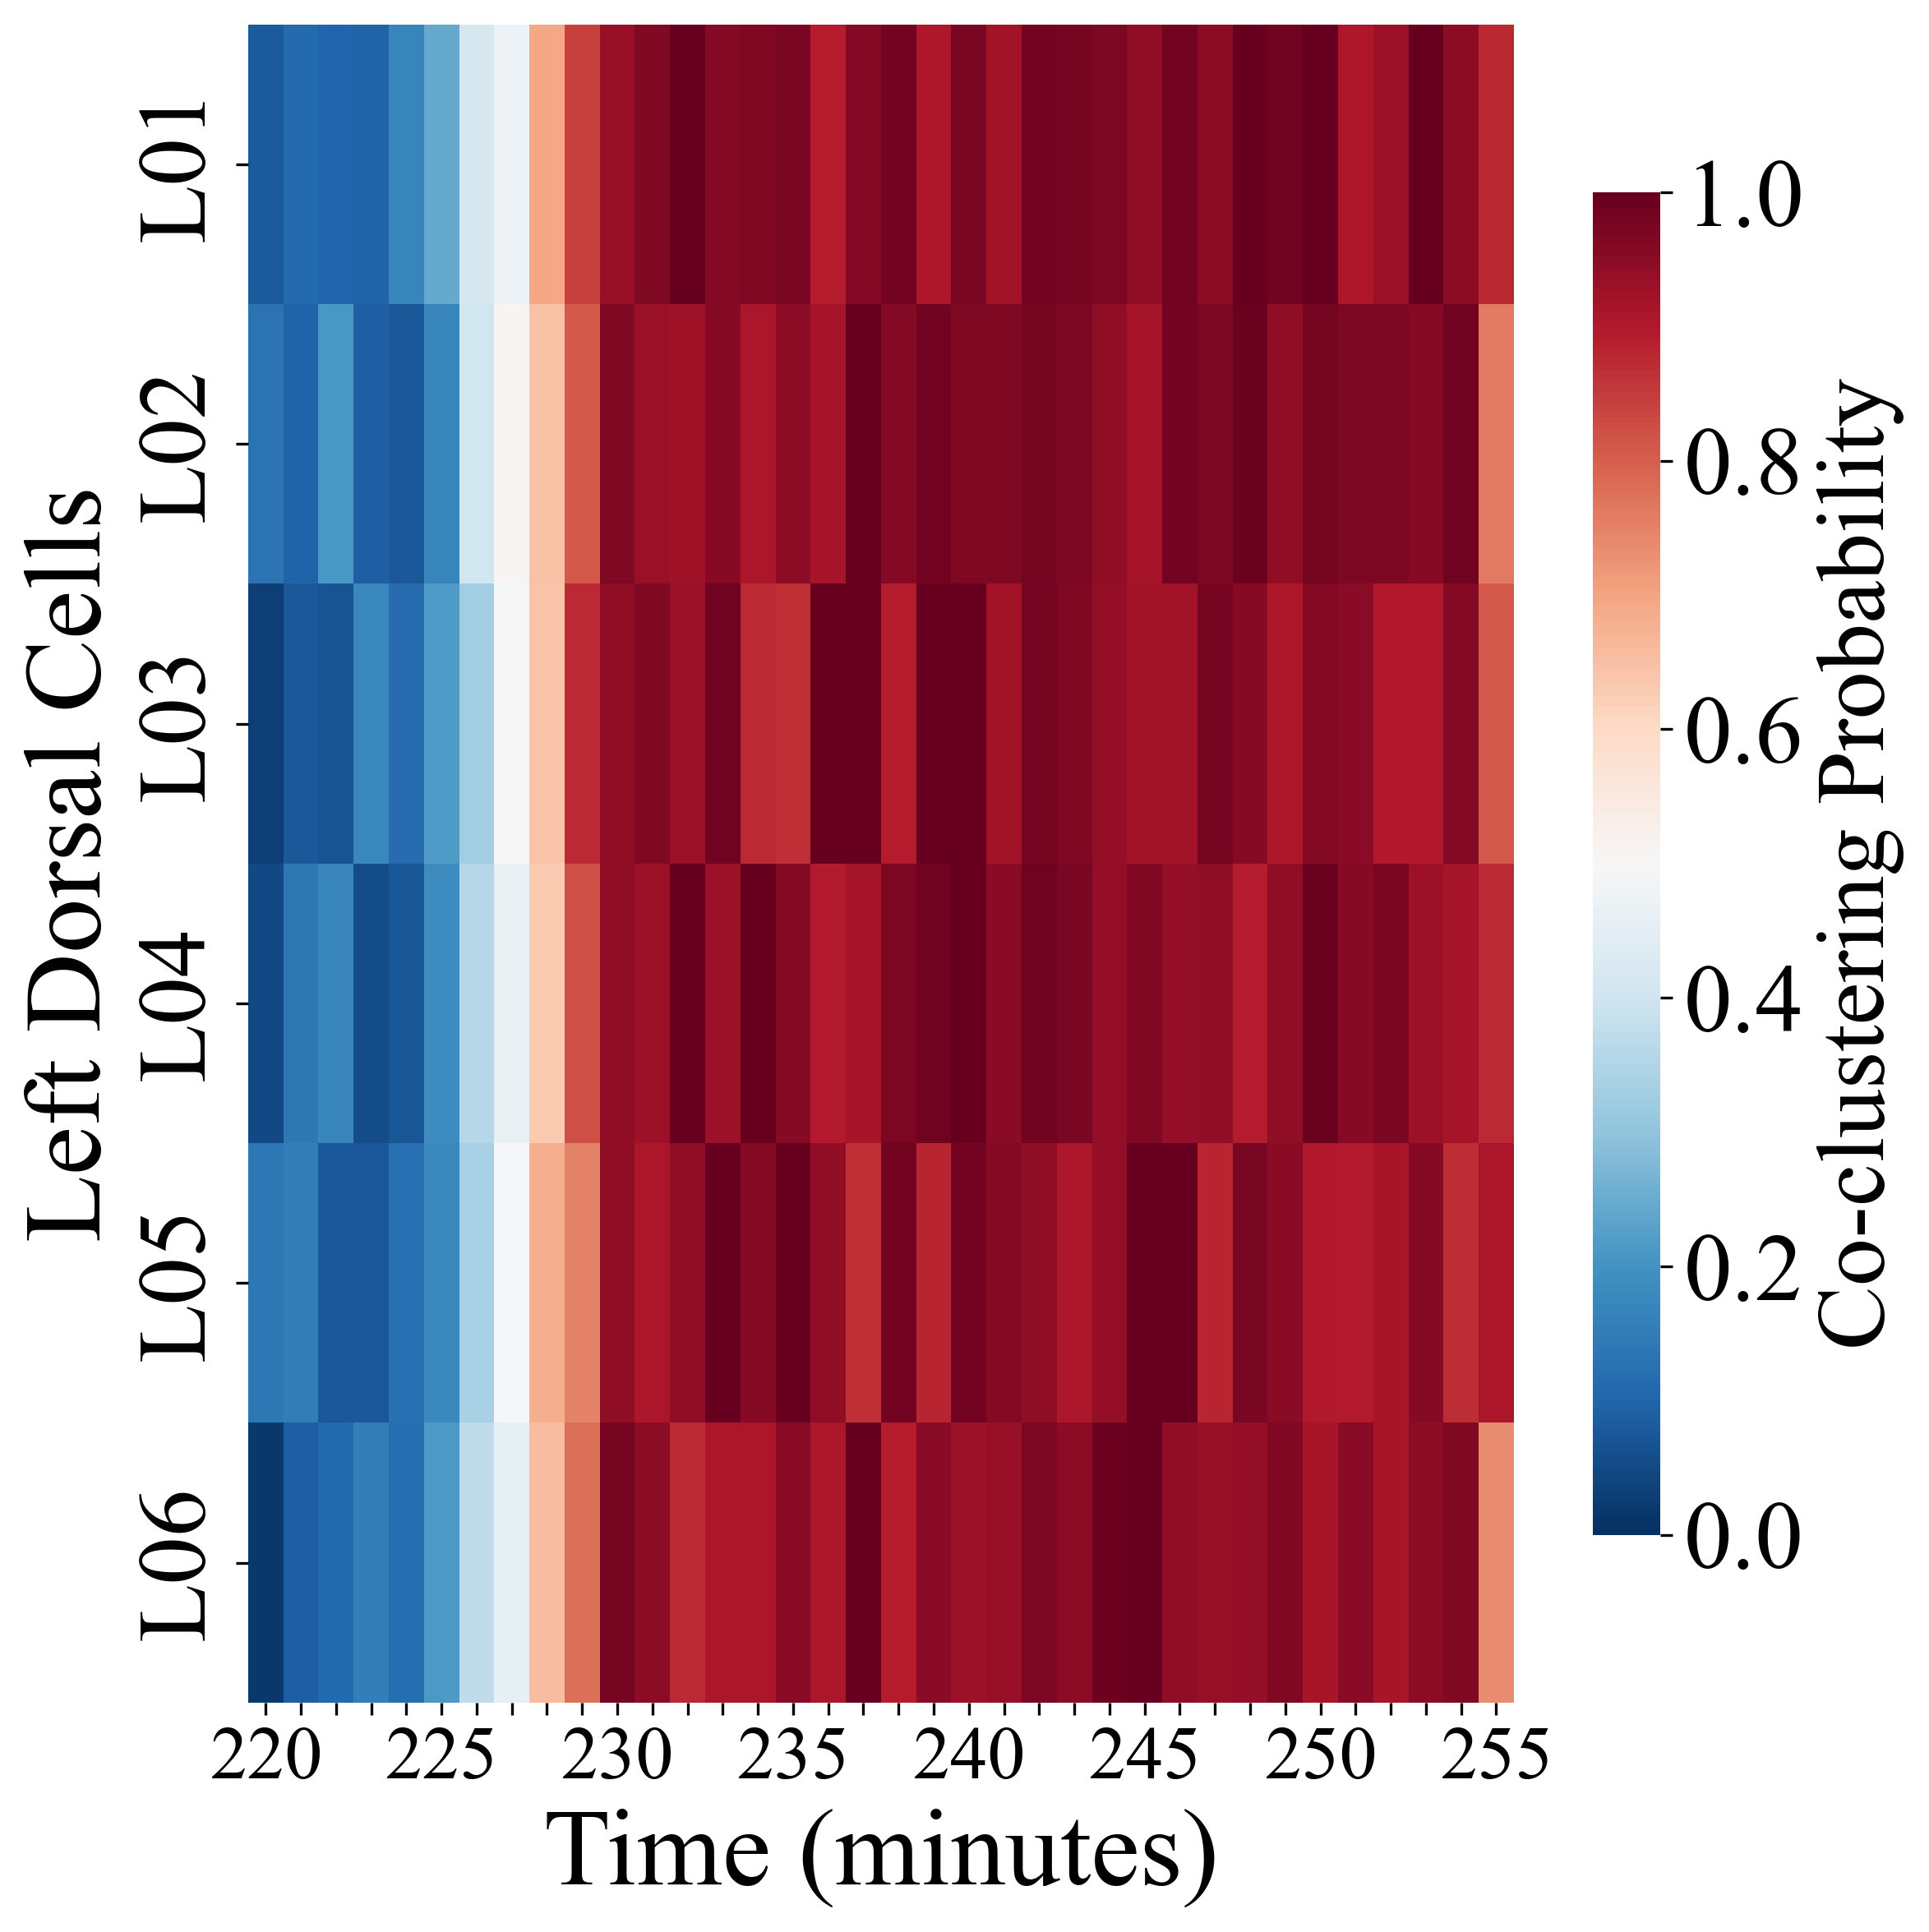
\includegraphics[width=\linewidth]{Demo1A_Dorsal_Left_Coclustering_Heatmap.png}
  \caption{\textbf{Dorsal Intercalation Left Side Co-clustering Heatmap.} Time-resolved co-clustering probability matrix for left-side dorsal intercalating cells during \textit{C.~elegans} embryonic morphogenesis (220--255 minutes post-fertilization). The heatmap displays pairwise clustering probabilities between 10 left-side hypodermal cells as they undergo convergent extension across the dorsal midline. High values (red) indicate synchronized clustering during 225--235 minutes; low values (blue) indicate independent movement. Cell identities correspond to hyp1L--hyp7L lineages.}
  \label{fig:di_left}
\end{figure}

\begin{figure}[t]
  \centering
  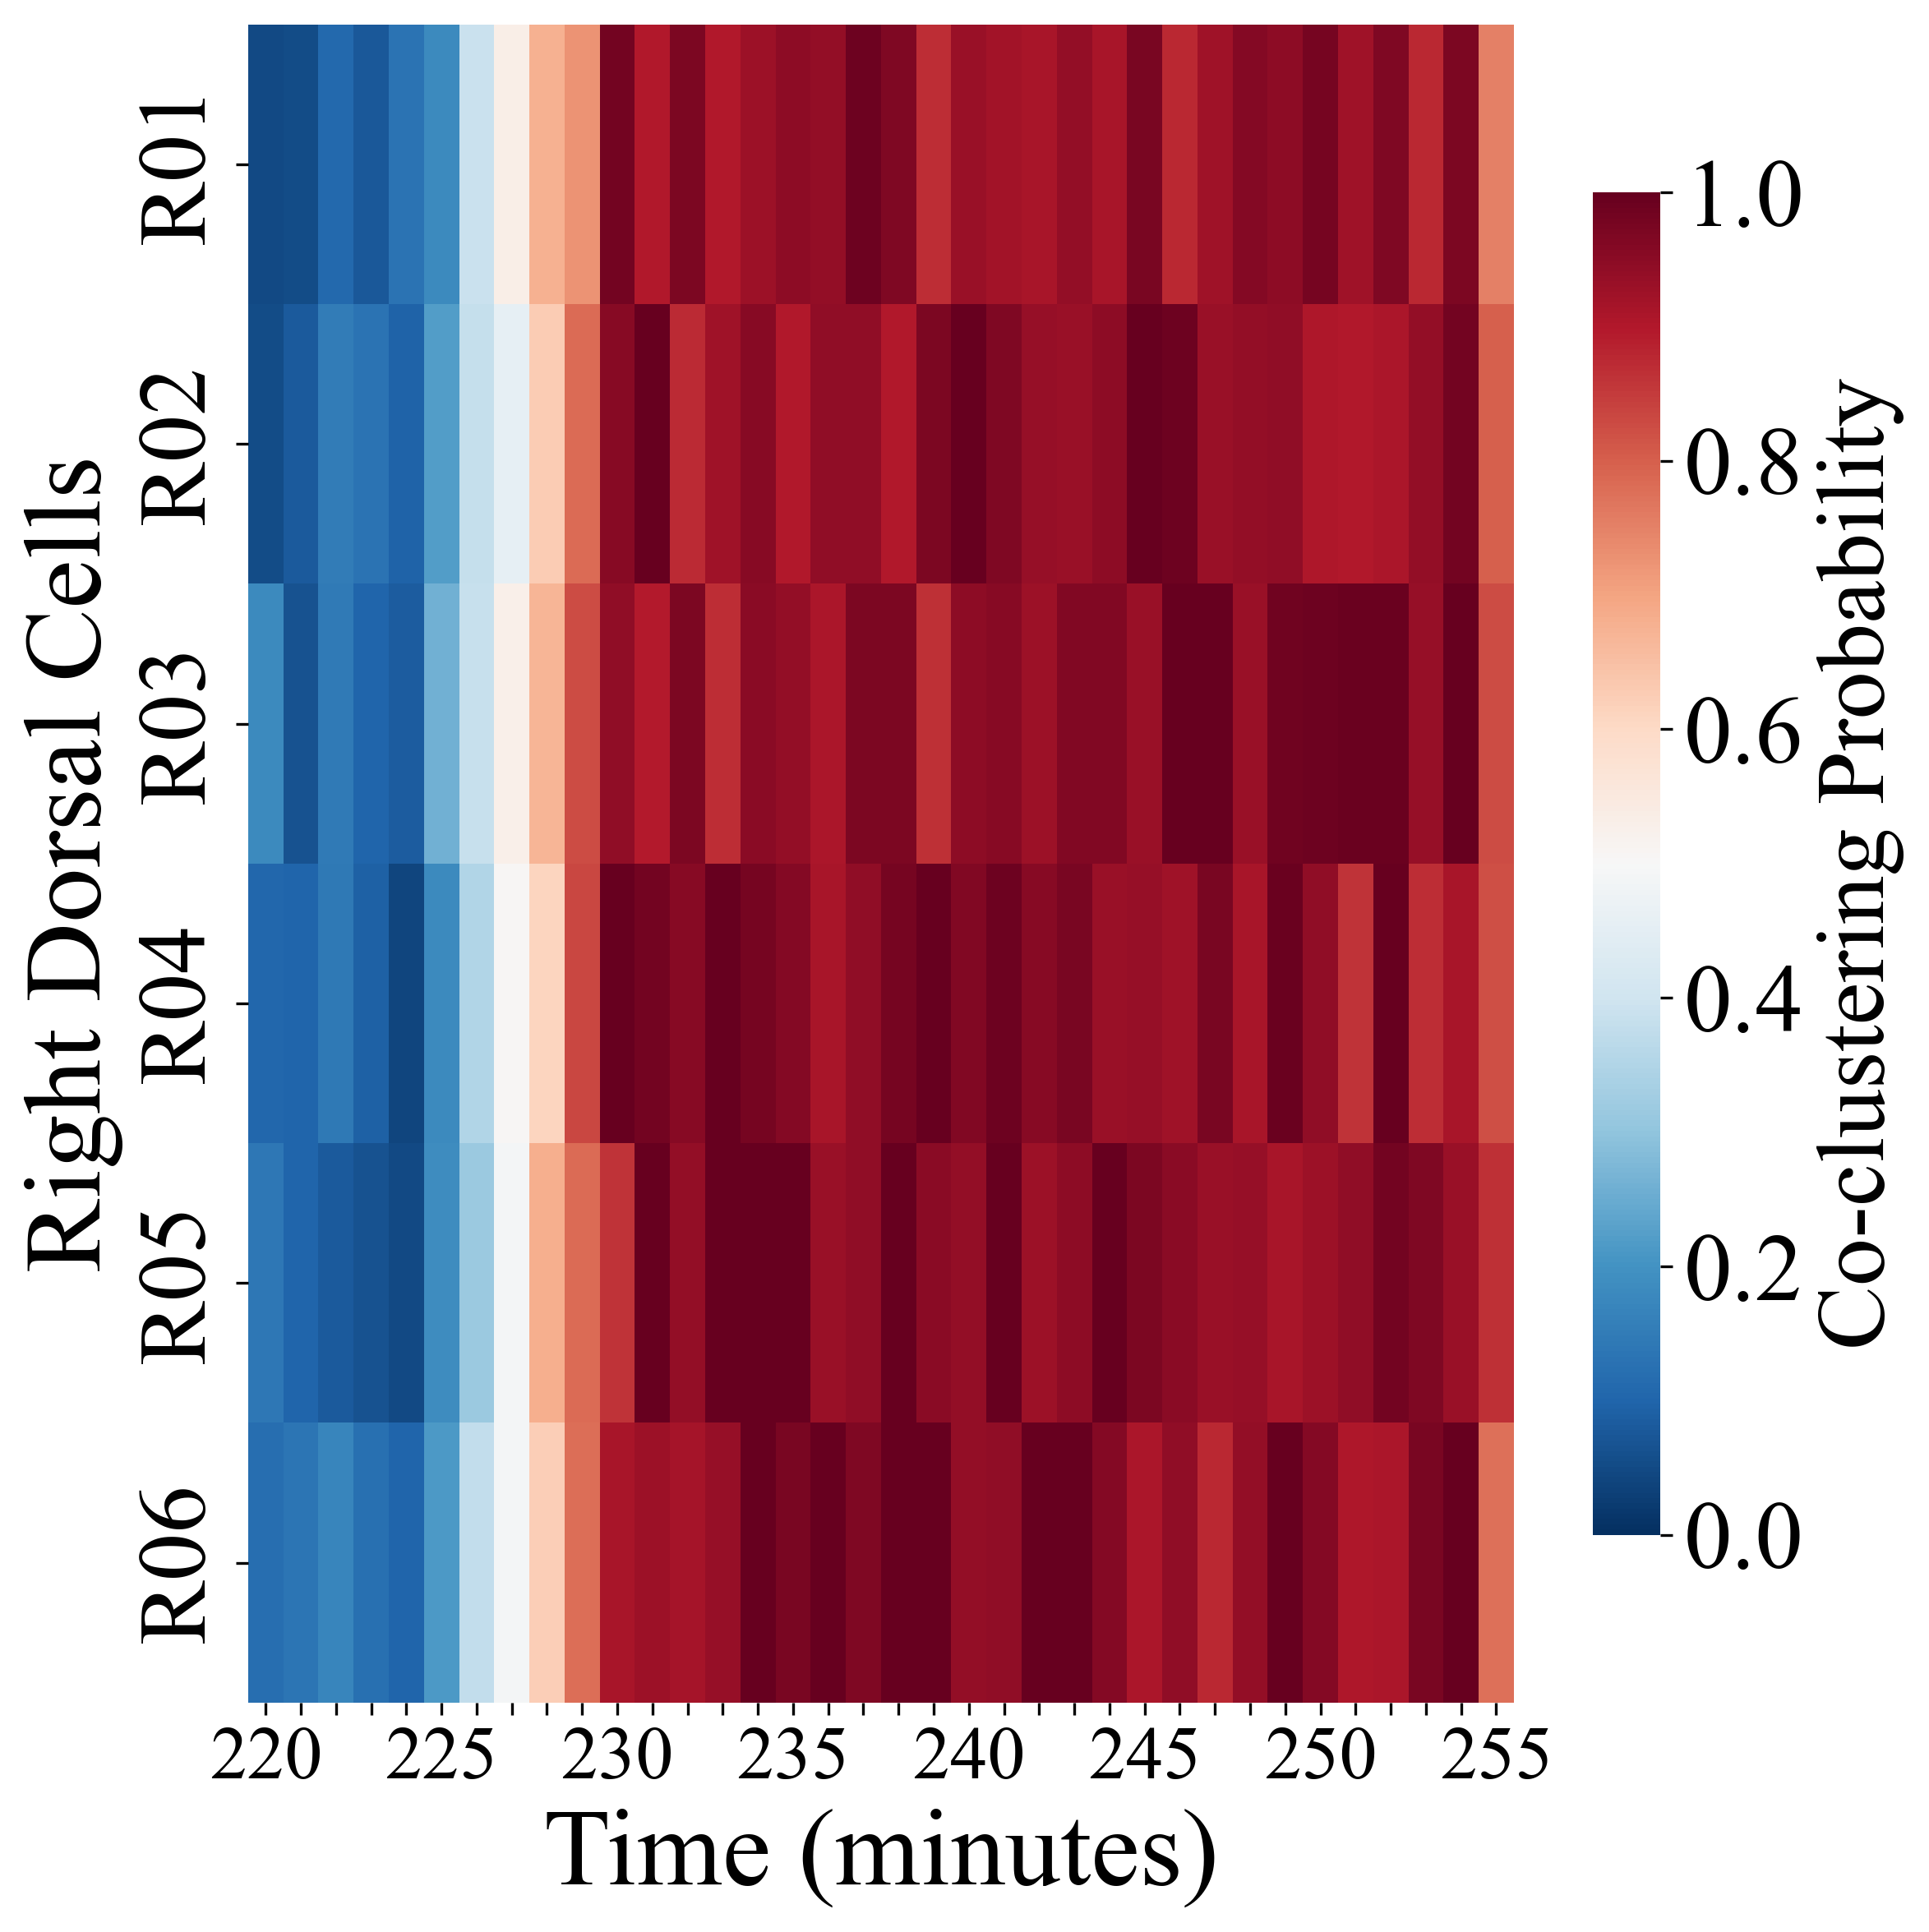
\includegraphics[width=\linewidth]{Demo1B_Dorsal_Right_Coclustering_Heatmap.png}
  \caption{\textbf{Dorsal Intercalation Right Side Co-clustering Heatmap.} Companion heatmap to Fig.~\ref{fig:di_left} for 10 right-side hypodermal cells (hyp1R--hyp7R). Peak co-clustering occurs during the window of basolateral protrusion extension and interdigitation across the midline.}
  \label{fig:di_right}
\end{figure}

\begin{figure}[t]
  \centering
  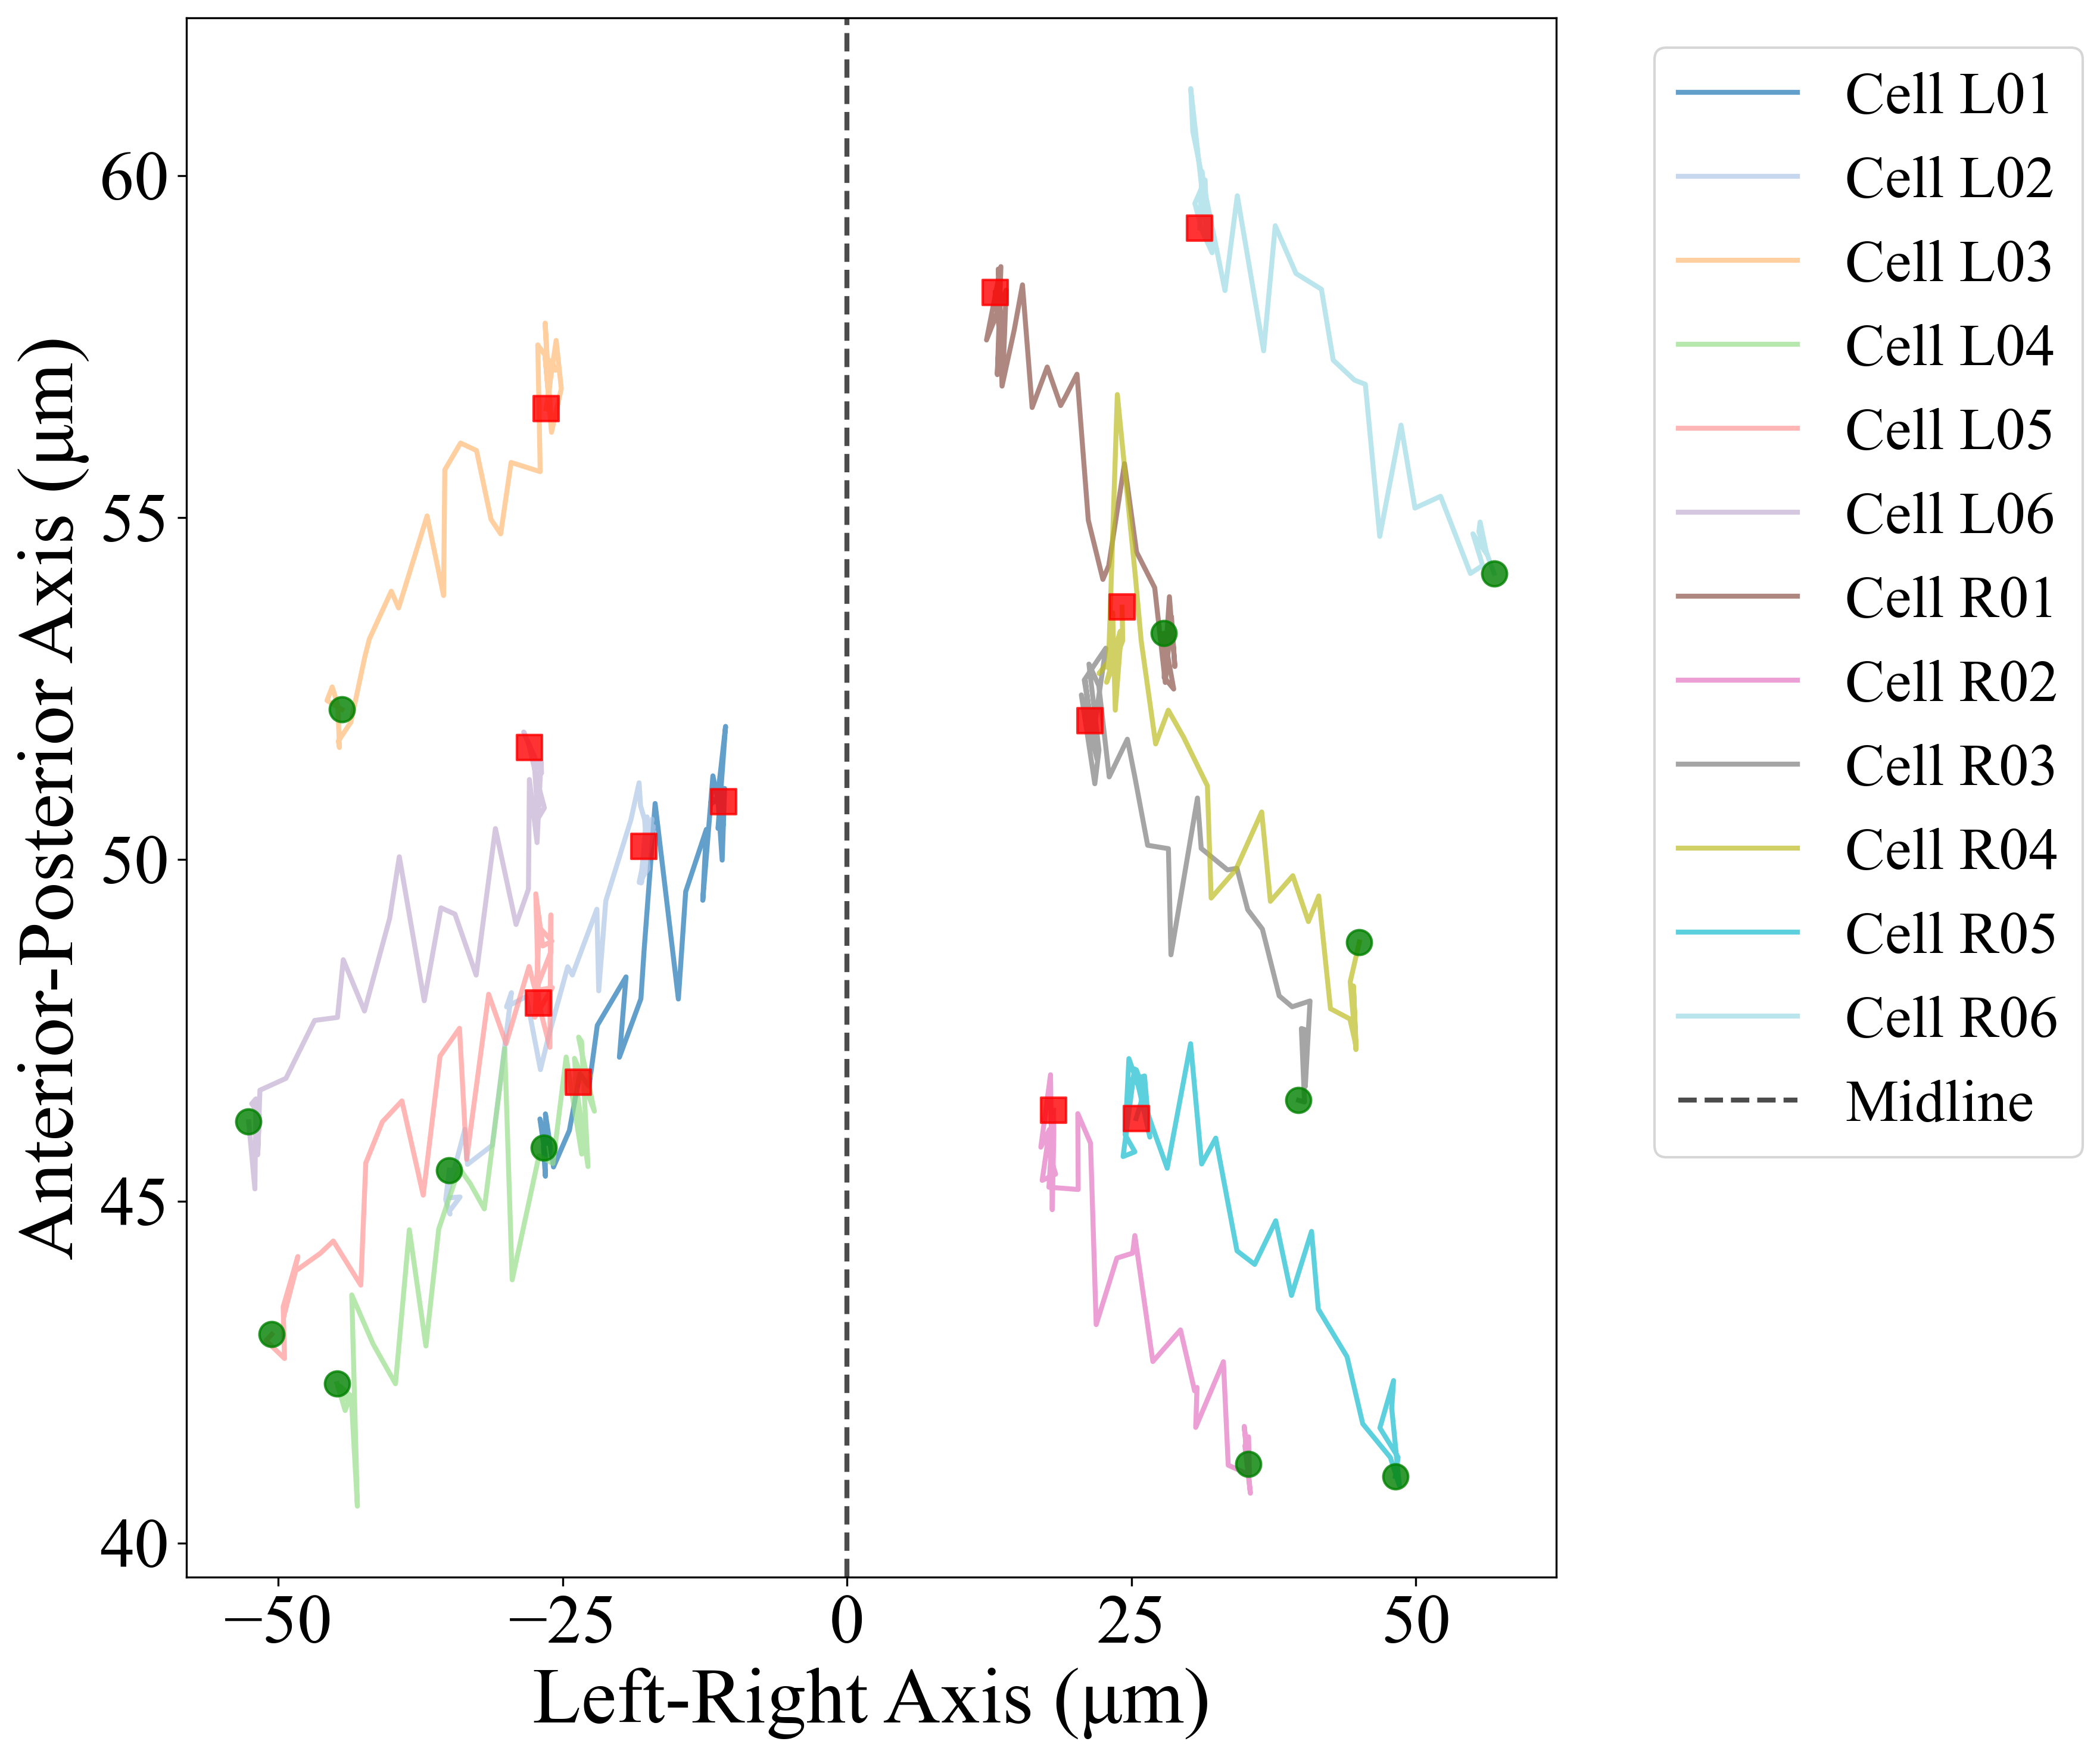
\includegraphics[width=\linewidth]{Demo2_Dorsal_Cell_Trajectories.png}
  \caption{\textbf{Dorsal Intercalating Cell Trajectories.} Spatial trajectories showing convergent extension: left (blue) and right (red) cohorts migrate toward the dorsal midline, exhibiting characteristic finger-like interdigitation. Axes denote anterior--posterior (x) and left--right (y).}
  \label{fig:di_tracks}
\end{figure}

\begin{figure}[t]
  \centering
  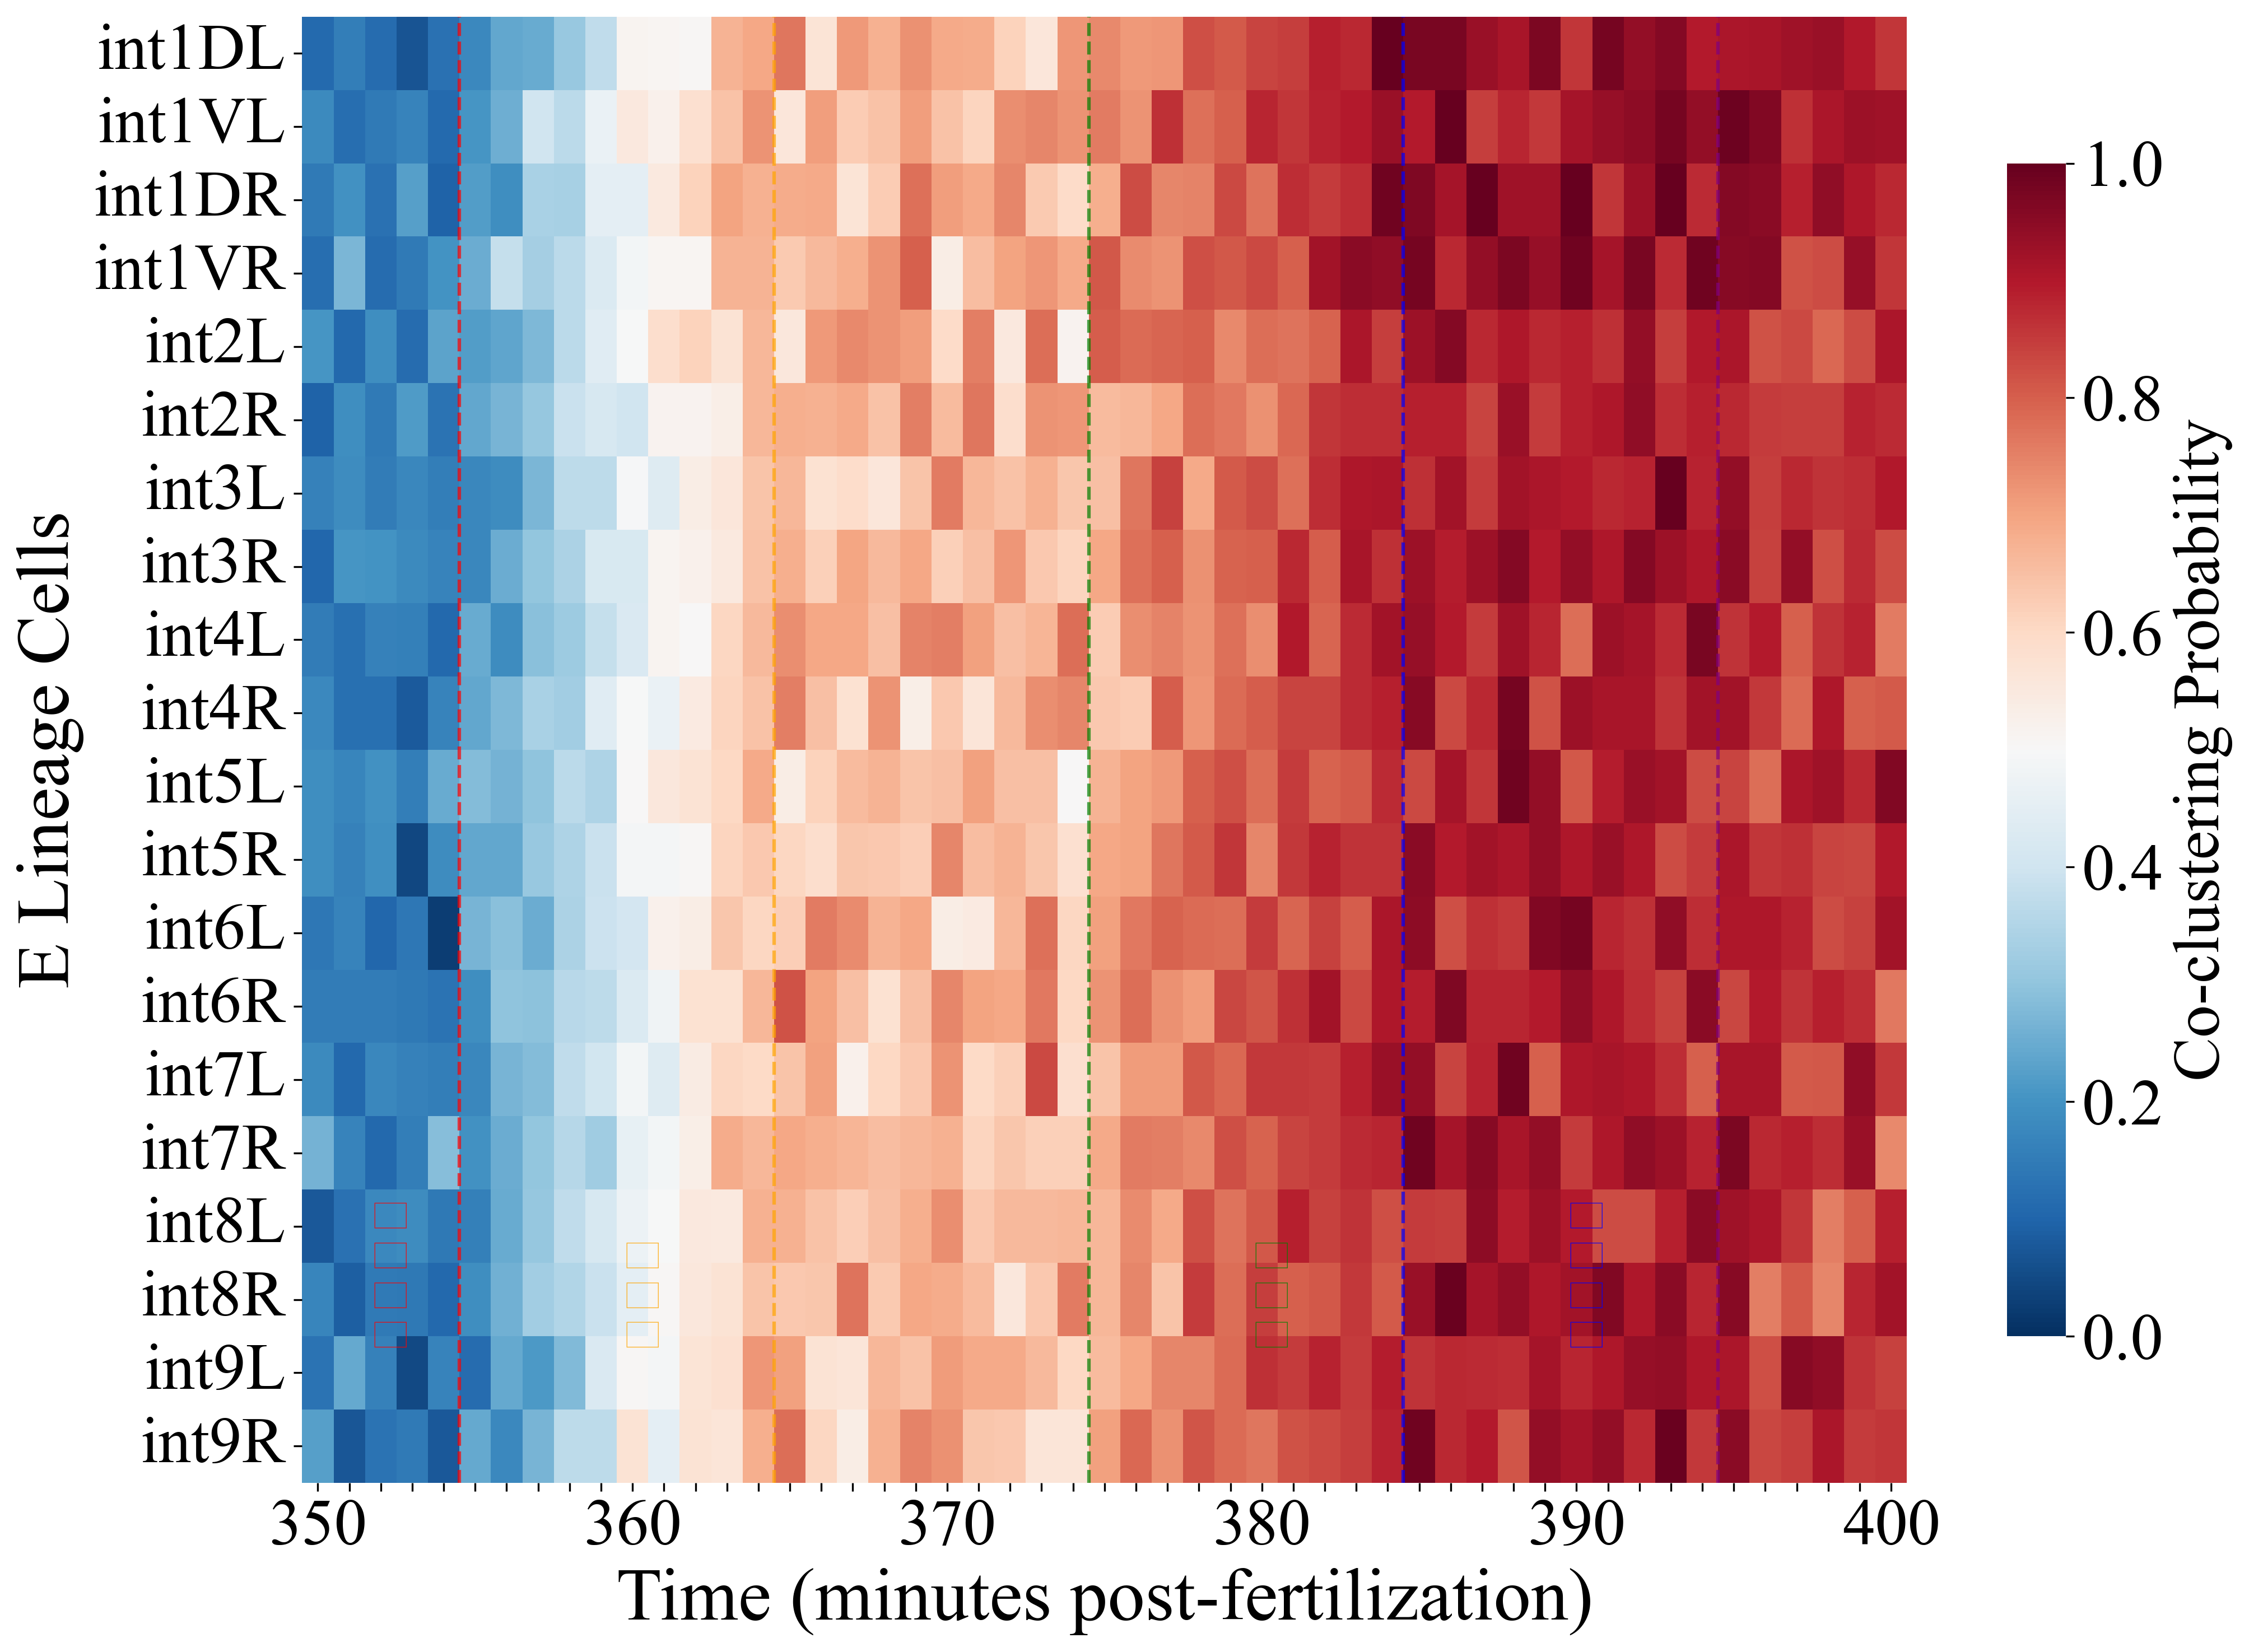
\includegraphics[width=\linewidth]{Demo4_Intestinal_Coclustering_Heatmap.png}
  \caption{\textbf{Temporal Decline Co-clustering Heatmap.} Co-clustering probability matrix for 12 dorsal cells (C01--C12) showing uniform high coordination during 225--240 minutes (red), followed by systematic decline during 240--255 minutes (blue), consistent with post-intercalation stabilization.}
  \label{fig:decline}
\end{figure}

\begin{figure}[t]
  \centering
  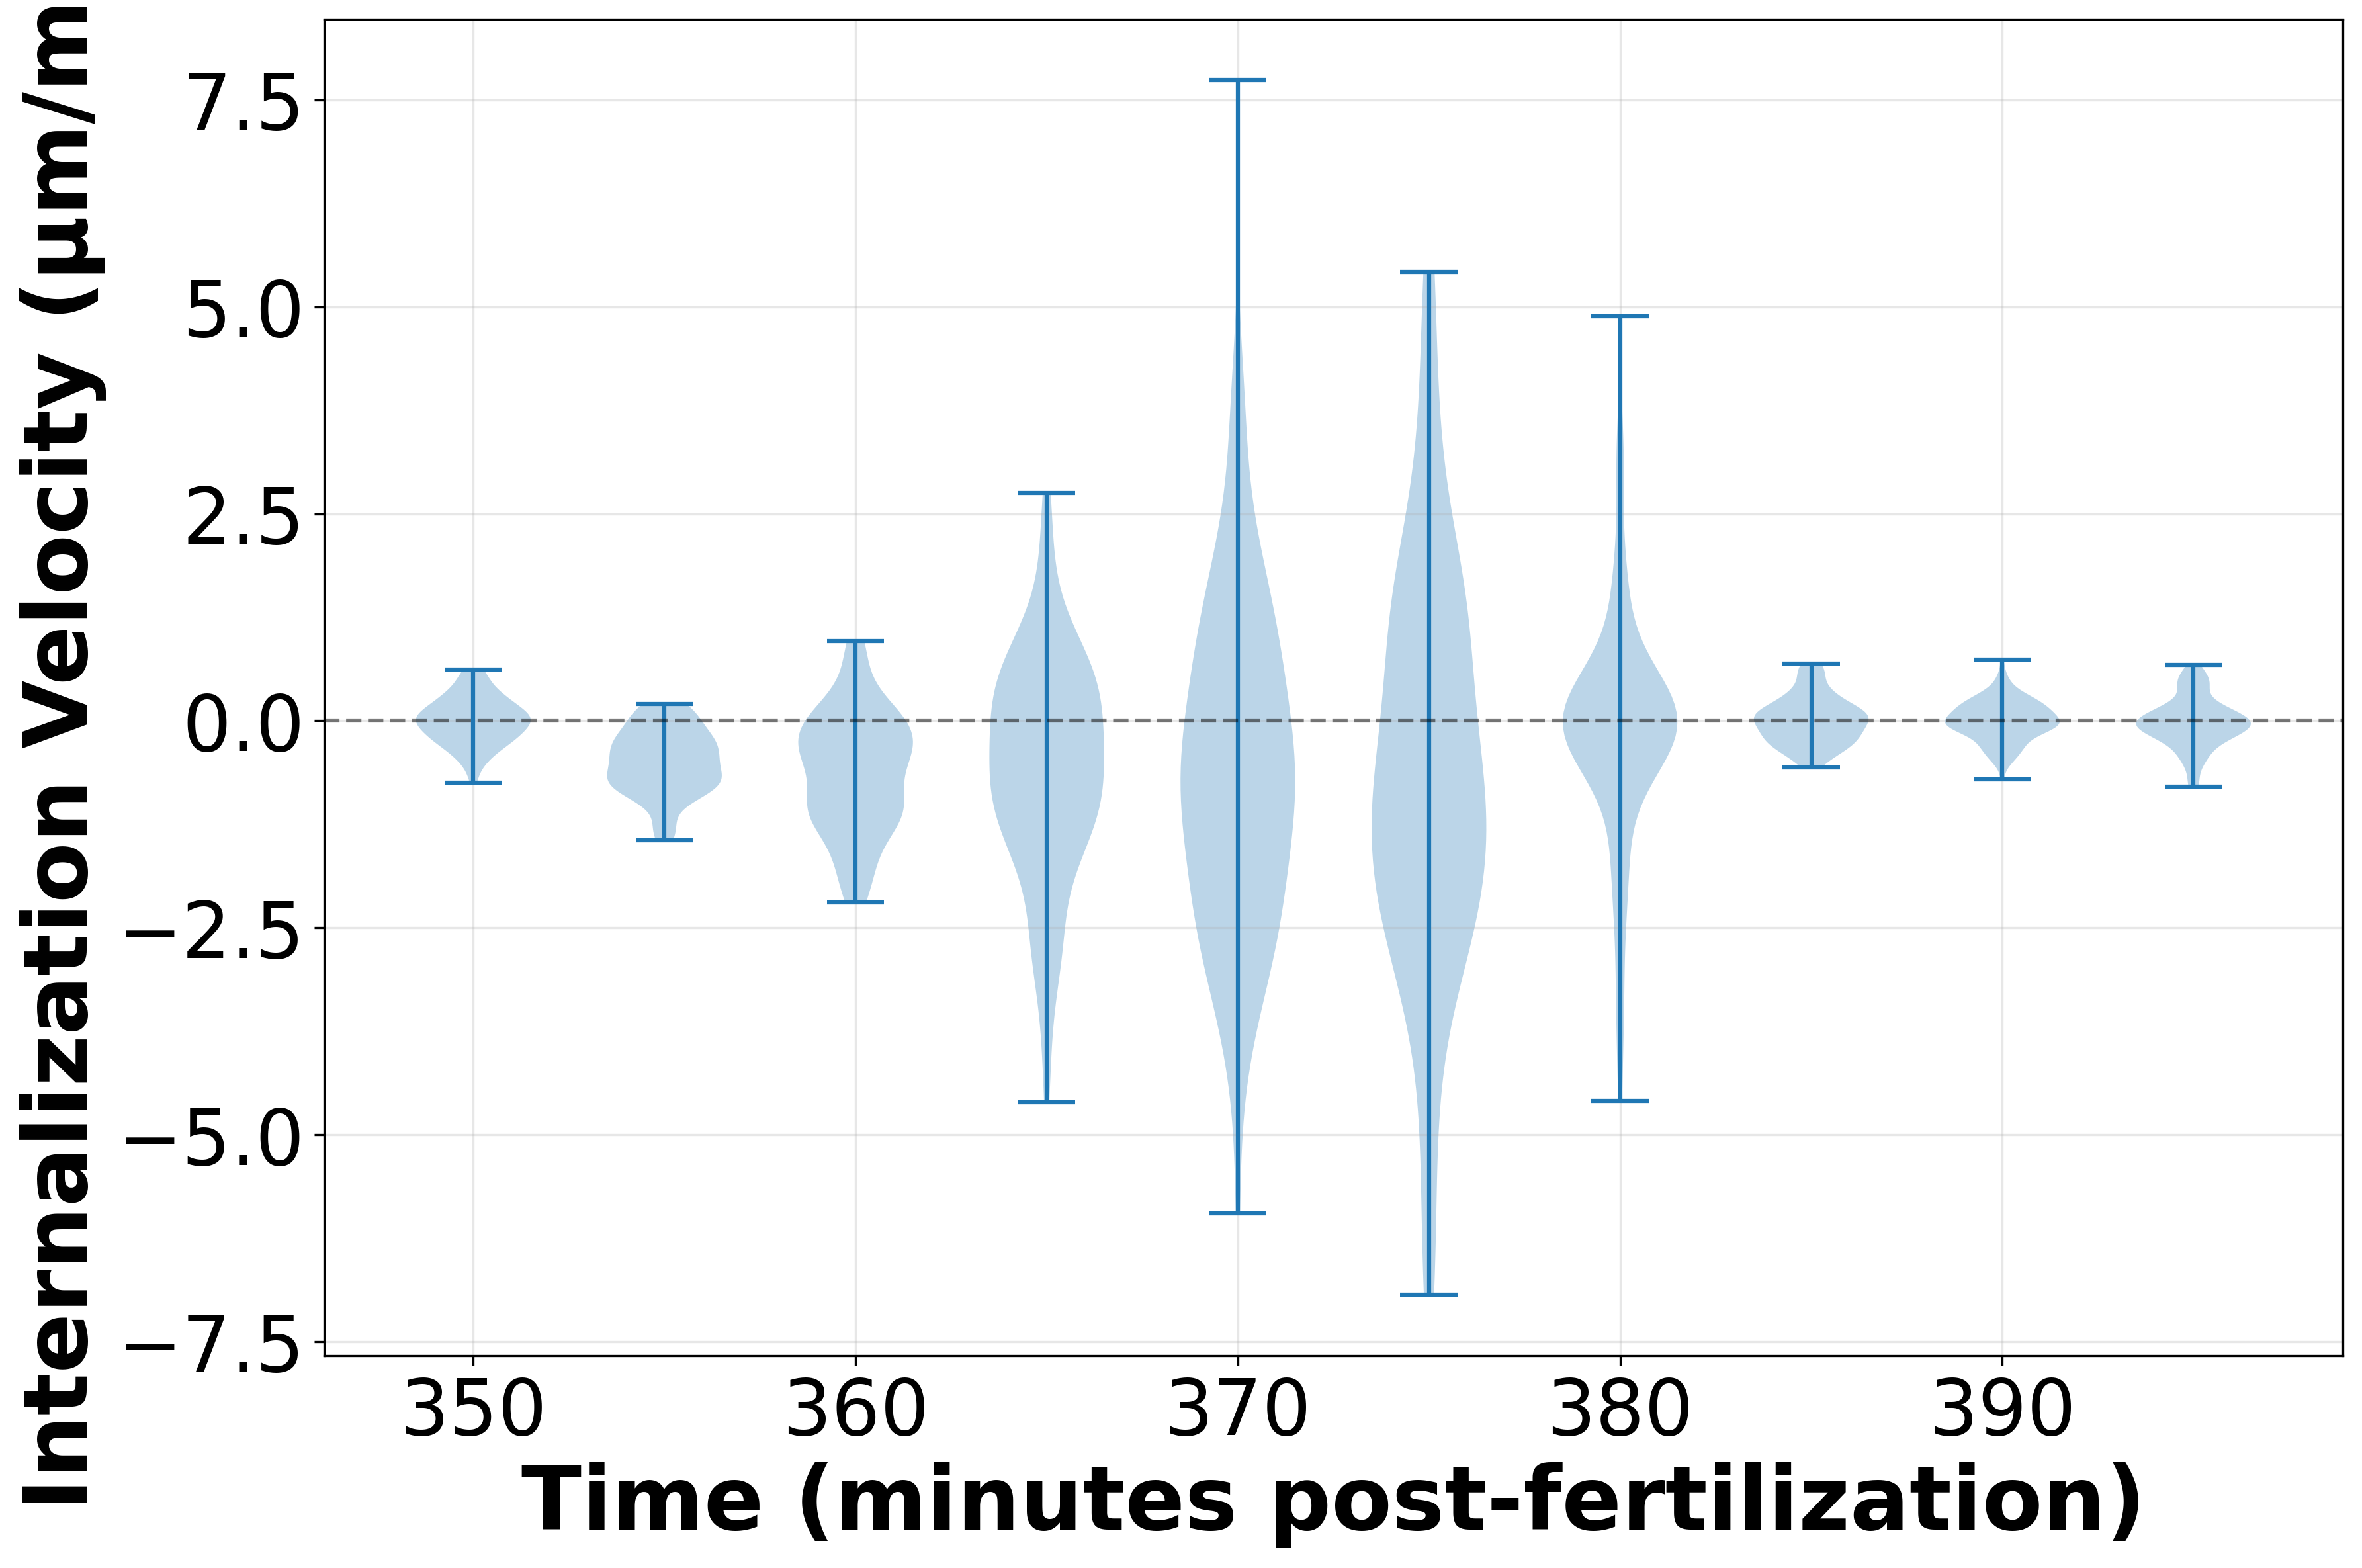
\includegraphics[width=\linewidth]{Demo6_Intestinal_Velocity_Field.png}
  \caption{\textbf{Intestinal Morphogenesis Velocity Field Analysis.} Velocity field of intestinal primordium cells during reorganization. Predominant negative $z$-velocities reflect inward movements associated with apical constriction and internalization; dynamics align with left--right asymmetry establishment and homotypic intercalation.}
  \label{fig:int_velocity}
\end{figure}

\begin{figure*}[t]
  \centering
  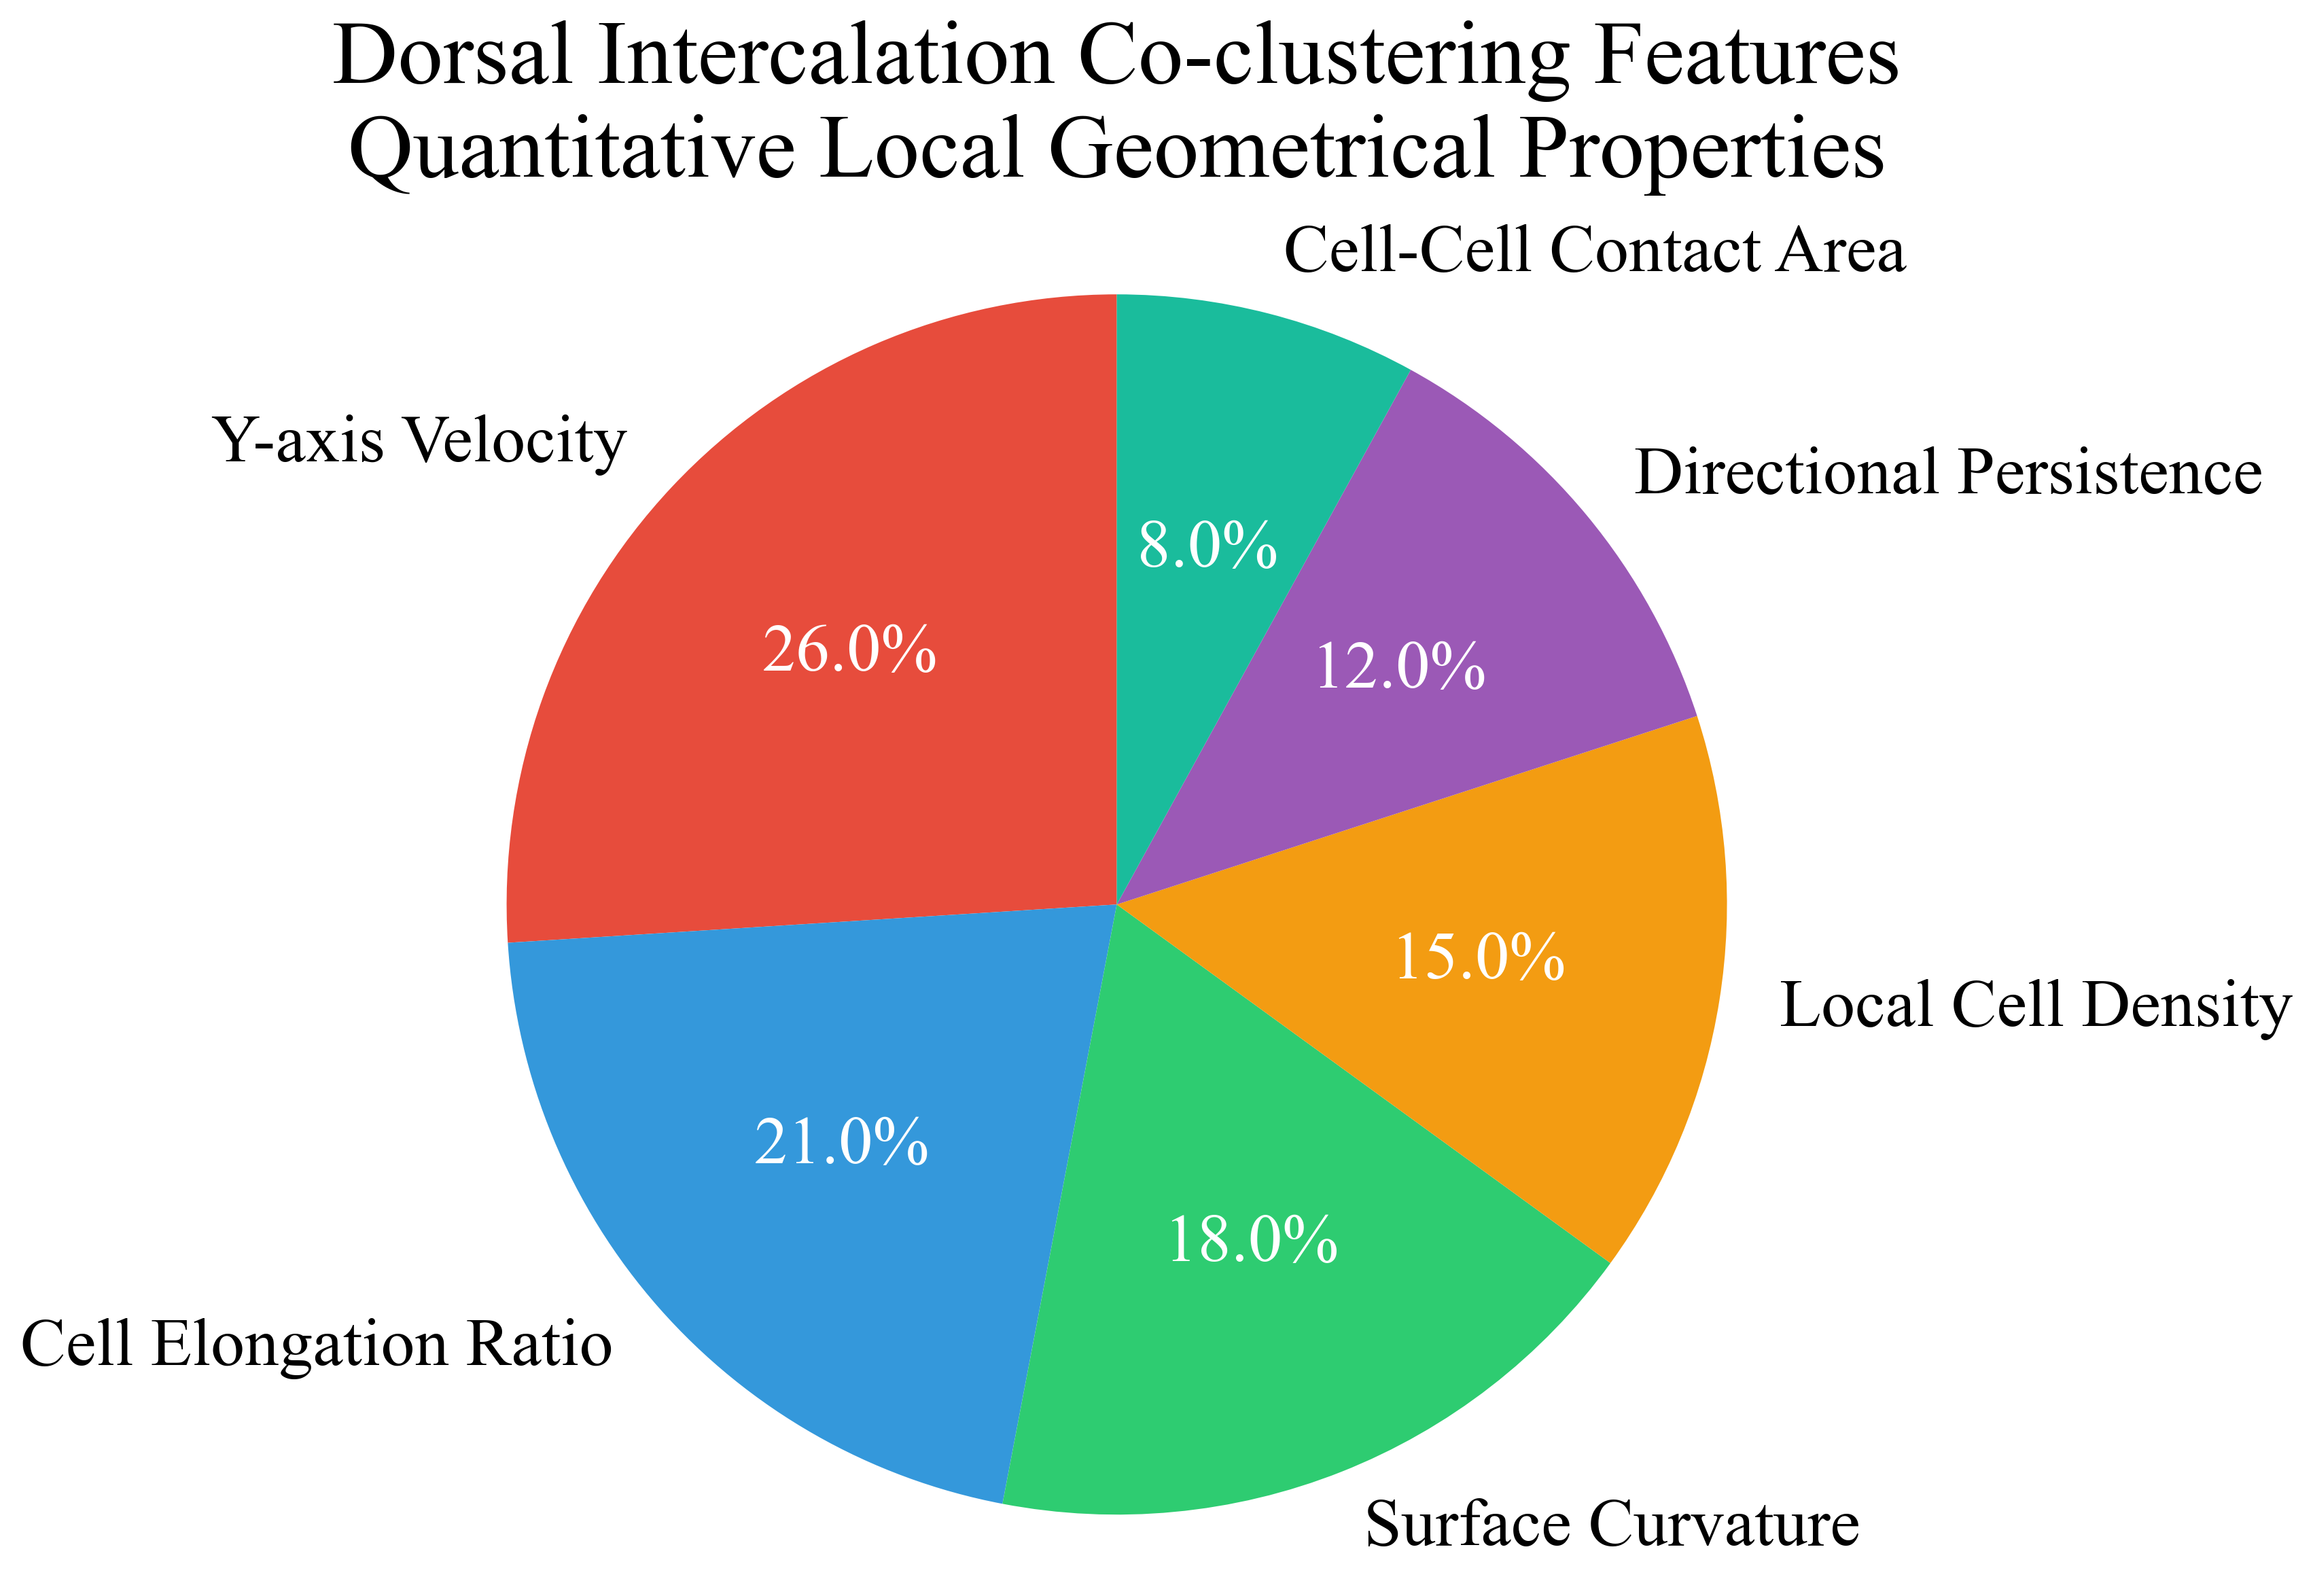
\includegraphics[width=.48\linewidth]{Demo7A_Dorsal_Coclustering_Features_Pie.png}\hfill
  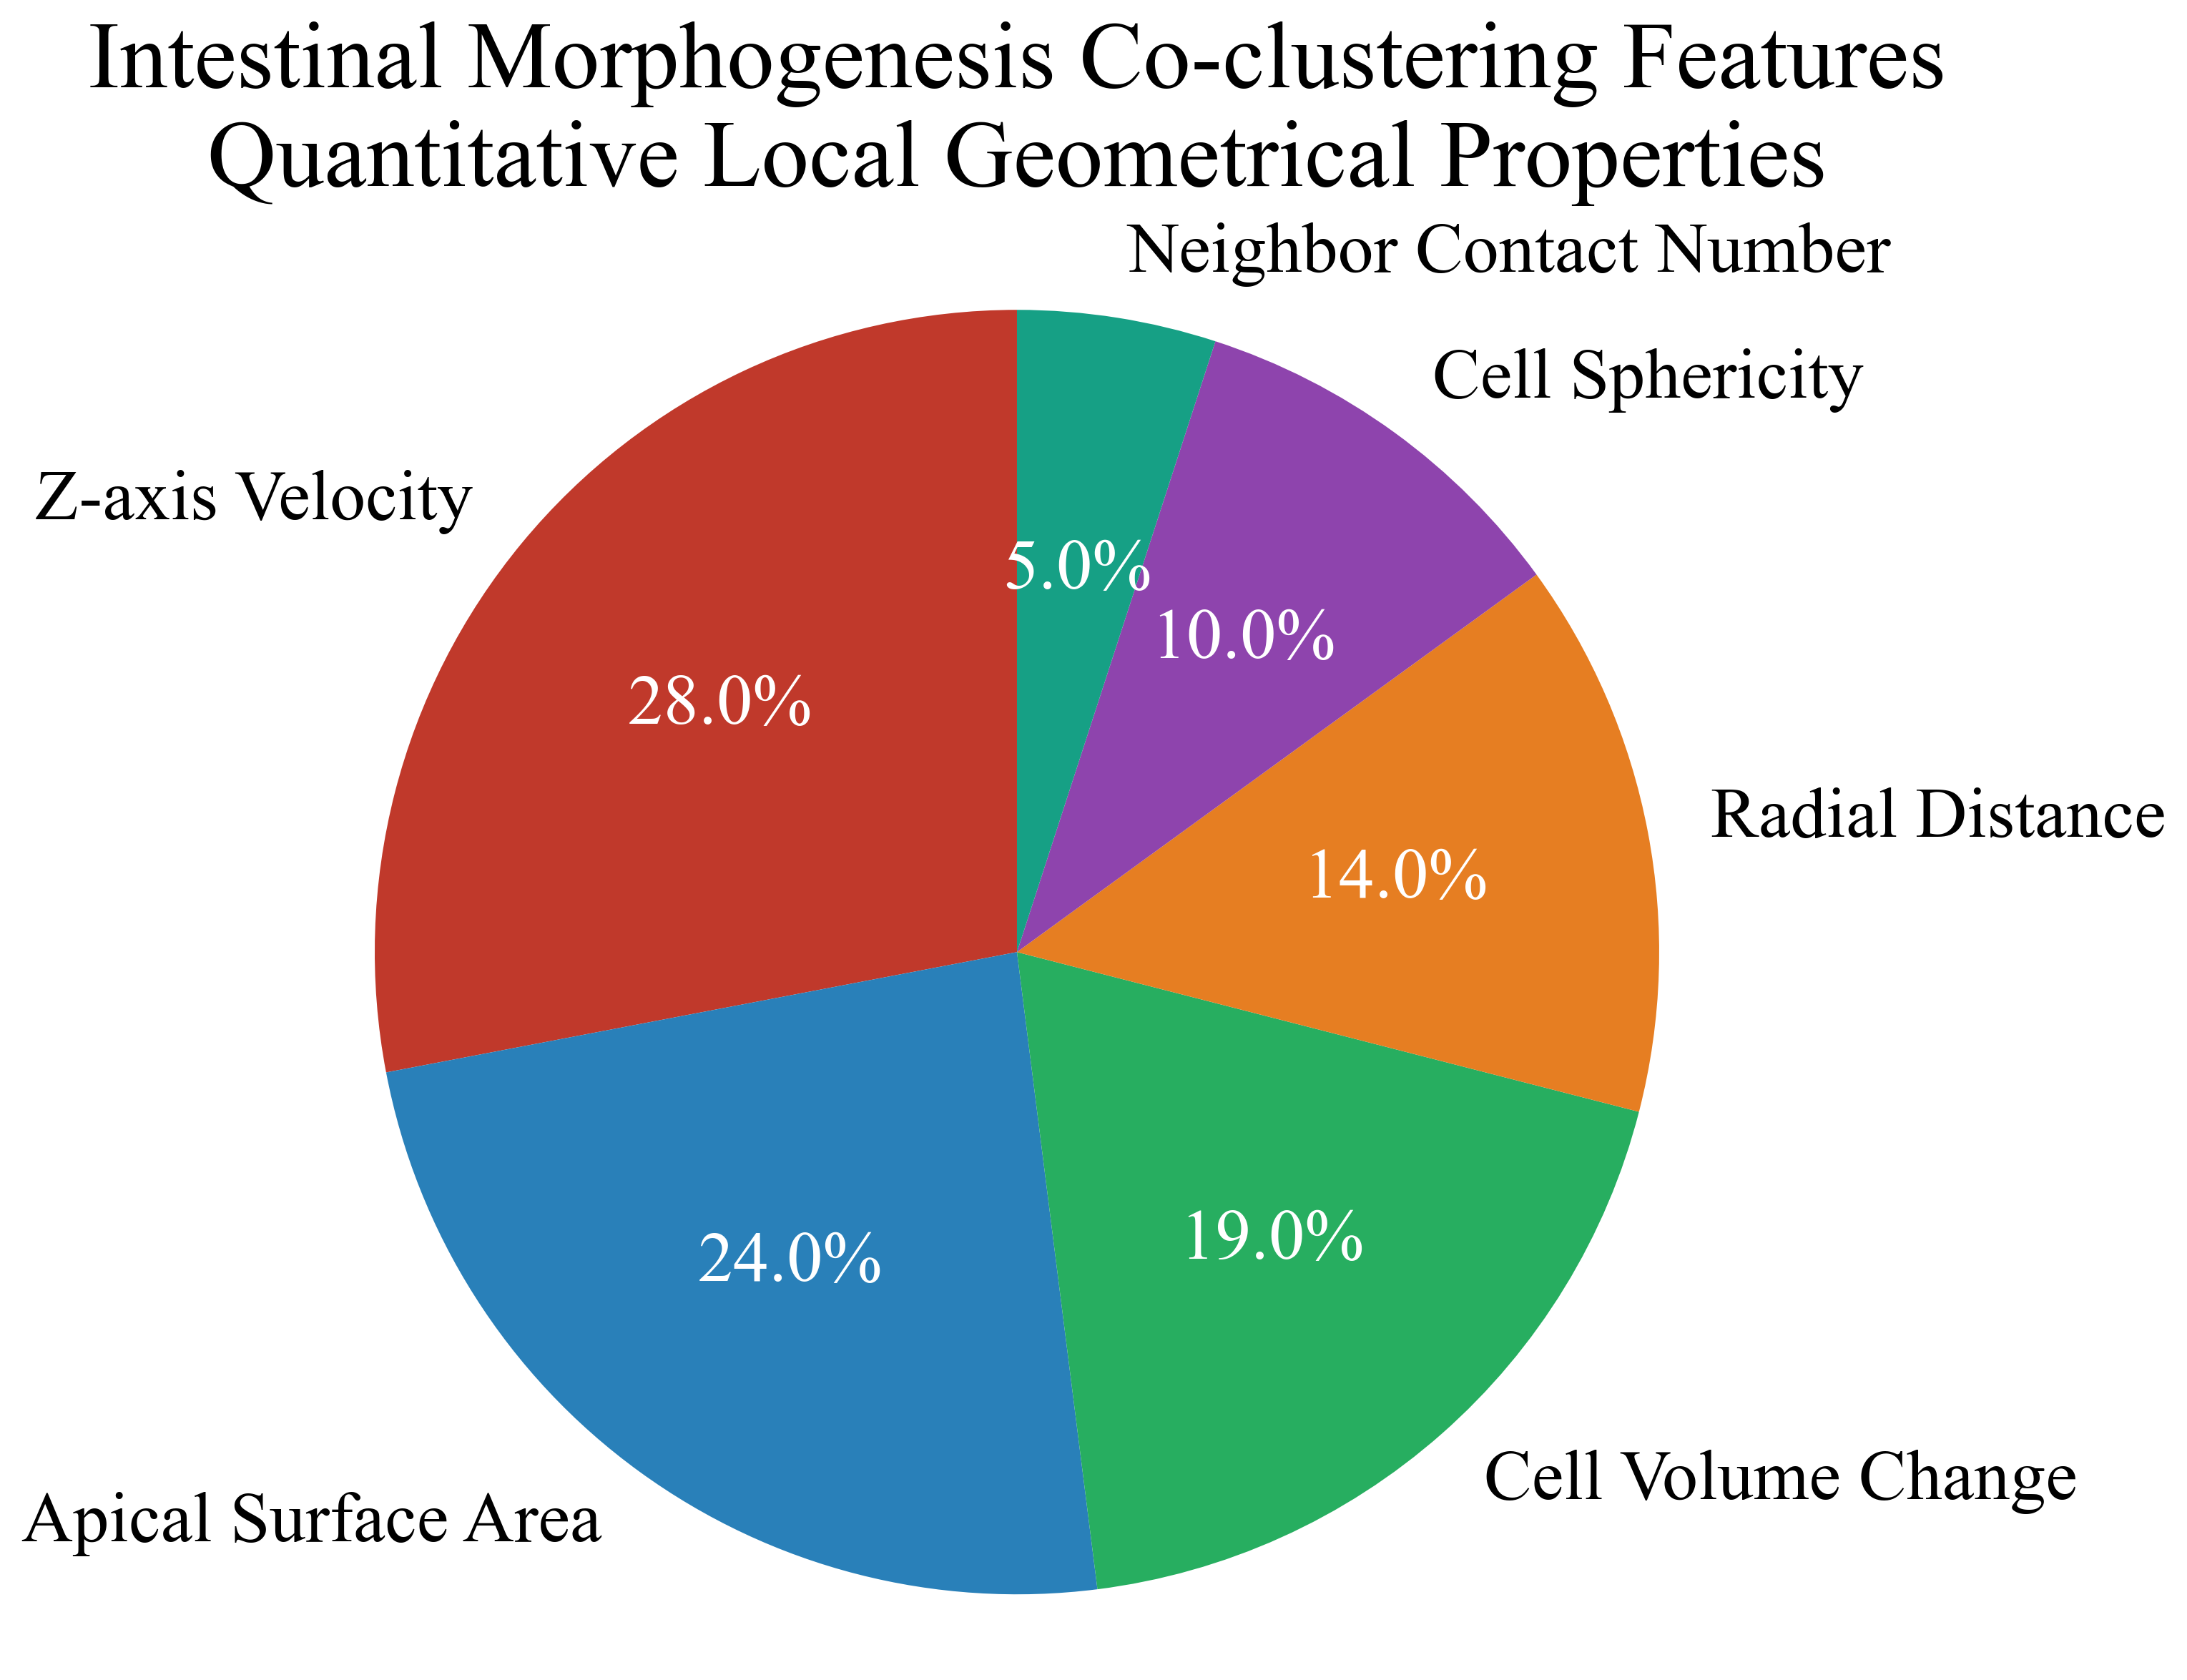
\includegraphics[width=.48\linewidth]{Demo7B_Intestinal_Coclustering_Features_Pie.png}
  \caption{\textbf{Morphogenetic Feature Distributions.} (\textbf{A}) Dorsal intercalation: relative weights indicate Y-velocity (26\%), cell elongation (21\%), surface curvature (18\%), and additional geometric features. (\textbf{B}) Intestinal morphogenesis: Z-velocity (28\%), apical surface area (24\%), volume change (19\%), and ancillary parameters. Weights derived from blockwise variance contributions (Eq.~\ref{eq:feature_weight}).}
  \label{fig:features}
\end{figure*}

% ------------------------ FUTURE WORK ------------------------
\section{Future Work: Careful Discovery of New Spatiotemporal Patterns}
\label{sec:future}

Our results indicate that tensor co-clustering can recover established behaviors in
\textit{C.~elegans}.  The next stage is to use the same framework, with stronger controls,
to discover \emph{previously unreported} patterns both in nematode embryogenesis and in
other systems.  Below we outline a cautious, extensible agenda.

\subsection{Guiding principles and discovery protocol}
We adopt a three-phase loop: (i) \emph{unsupervised discovery} under strict regularization,
(ii) \emph{pre-registered testing} on held-out embryos or perturbations, and
(iii) \emph{mechanistic triangulation} by orthogonal readouts (e.g., genetics, force or
signaling reporters).  Concretely:
\begin{enumerate}
  \item \textbf{Candidate generation.} Run DiMergeCo on standardized tensors
  $\mathcal{X}\in\mathbb{R}^{C\times T\times F}$ with multiple random partitions
  and hierarchical merges.  Retain only tri-clusters $\mathcal{B}_u$
  with high stability across runs (consensus Jaccard $\geq \tau$).
  \item \textbf{Statistical vetting.} For each candidate block $u$ with index sets
  $(\mathcal{I}_u,\mathcal{J}_u,\mathcal{K}_u)$, compute a block score $S_u$ (variance
  explained and cross-mode coherence).  Estimate a null by (a) blockwise circular
  time-shifts, (b) feature knockoffs within embryos, and (c) lineage-preserving
  label permutations.  Control the false discovery rate (FDR) across all $u$ by the
  Benjamini–Yekutieli procedure, or by knockoff+ thresholds when feature dependence is strong.
  \item \textbf{Out-of-sample confirmation.} Freeze hyperparameters and evaluate the same
  motifs on embryos not used in discovery or on specific perturbations.  Report calibrated
  $p$-values or posterior inclusion probabilities together with uncertainty intervals.
\end{enumerate}
To make uncertainty explicit, we will extend the framework with a Bayesian layer that
places a prior on the number and size of blocks and returns posterior credible sets for
$\{\mathcal{I}_u,\mathcal{J}_u,\mathcal{K}_u\}$.

\subsection{New pattern classes to search for in \textit{C.~elegans}}
We will focus on patterns that are plausible given current developmental theory but are
not yet formally catalogued at single-cell, minute-scale resolution.

\paragraph{(A) Micro-coordination waves during dorsal intercalation.}
Beyond the known midline crossing, test for short-latency \emph{phase-locked bands} of
cells with alternating high/low medial velocity.  Operationally, seek tri-clusters with
(i) narrow time windows ($\leq 5$--$8$ min), (ii) alternating sign of velocity divergence
across the left/right cohorts, and (iii) elevated directional persistence.  As a
pre-registered falsification, require disappearance of this motif under actin
disruption, but not under microtubule attenuation.

\paragraph{(B) Leader–follower switches.}
Identify tri-clusters where the ordering of peak speed or elongation between two or more
cells reverses within a single interdigitation event.  Quantify with a Kendall-$\tau$
time-course computed within $\mathcal{J}_u$.  A robust pattern must (i) recur across
embryos, (ii) survive time-warp alignment (DTW) to a dorsal-closure clock, and
(iii) show lineage symmetry (left/right analogs).

\paragraph{(C) Pre-closure tension release.}
Search for transient drops in curvature-derived strain proxies immediately after high
co-clustering epochs---a signature of mechanical relaxation.  Couple DiMergeCo with
change-point detection: test whether the block-average feature vector
$\bar{\mathbf{x}}_u(t)$ has a statistically significant break at $t^\star$ with
HAC-corrected confidence.

\paragraph{(D) Rare, lineage-restricted microstates.}
Use scan statistics over small $|\mathcal{I}_u|$ and short $|\mathcal{J}_u|$ together
with Poisson-binomial nulls to detect rare but repeated microstates (e.g., brief apical
surface pulses).  Require replication across embryos and robustness to 10--20\% synthetic
missingness.

\subsection{Beyond \textit{C.~elegans}: comparative and translational extensions}
The tensor design is agnostic to species; only feature dictionaries and alignment change.

\paragraph{(E) Gastrulation in \textit{Drosophila}.}
Construct $\mathcal{X}$ from cell patches during ventral furrow formation; features include
apical area, anisotropy, myosin reporter intensity, and tissue flow invariants
(divergence, shear).  Hypothesis: DiMergeCo will isolate medio-lateral \emph{shear bands}
and apical constriction \emph{phase fronts}.  Validate against optogenetic perturbations.

\paragraph{(F) Zebrafish epiboly and convergence/extension.}
Use nuclei tracking to form cell--time--(velocity/neighbor) tensors.  Search for tri-clusters
that couple \emph{planar cell polarity} alignment with region-specific strain rates.
Confirm with PCP mutants as negative controls.

\paragraph{(G) Mouse peri-implantation and early streak.}
Apply a multi-embryo atlas with optimal-transport alignment to a common morphospace; add
signaling reporters (e.g., Wnt, Nodal) as an auxiliary feature mode.  Look for
tri-clusters that link morphodynamic states to signaling pulses; test directionality by
time-lagged Granger-style regressions with block bootstraps.

\paragraph{(H) Organoids and in~vitro epithelia.}
In intestinal and brain organoids, combine 3D shape descriptors (sphericity, curvature,
surface Laplacian) with lumen volume and polarity markers.  Search for tri-clusters that
predict lumen collapse or symmetry breaking; prospectively validate by microfluidic
osmolarity shifts.

\paragraph{(I) Collective cell migration and wound healing.}
At tissue scale, let cells be \emph{patches} or superpixels.  Include kinematic
invariants (strain-rate tensor eigenvalues), traction forces (if available), and local
topology (Delaunay degree, T1/T2 transitions).  Hypothesis: DiMergeCo can separate
\emph{leader-ridge} bands from \emph{follower} sheets with distinct curvature/traction
profiles.

\subsection{Methodological developments to reduce false positives}
To safely expand discovery, we plan the following technical additions.

\paragraph{(M1) Bayesian and uncertainty-aware co-clustering.}
Introduce a posterior over blocks with sparsity and contiguity priors across $T$.
Report for each cell--time pair a marginal inclusion probability $\pi_{it}$ and adopt
a calibrated threshold (e.g., controlling the Bayesian FDR).  Use Rao–Blackwellized
averages to stabilize feature weights $w_f$.

\paragraph{(M2) Physics-informed and topology-aware features.}
Augment the feature dictionary with (i) 3D kinematic invariants (trace-free strain rate,
vorticity magnitude), (ii) tissue-scale transport (dynamic optimal transport costs), and
(iii) topological descriptors (persistent homology of cell–cell contact graphs).  Enforce
SE(3)-equivariance in learned features to avoid orientation artifacts.

\paragraph{(M3) Alignment across embryos and species.}
Before co-clustering, align time axes by dynamic time warping to a morphogenetic clock
and align spaces by Procrustes/optimal transport in a small set of \emph{anchor}
features.  Propagate alignment uncertainty into the co-clustering posterior.

\paragraph{(M4) Streaming, out-of-core, and federated scaling.}
Implement a streaming variant that updates local factors on minibatches and merges
periodically; analyze its regret relative to the full-batch solution.  For multi-site
data, use federated consensus co-clustering with secure aggregation and prove that the
communication complexity remains $O(\log P)$ in the number of sites $P$.

\paragraph{(M5) Rare-event sensitivity and scan statistics.}
Embed a multi-scale scan over $(|\mathcal{I}|,|\mathcal{J}|)$ with exact or saddlepoint
$p$-values to detect small, transient motifs, while controlling familywise error under
strong dependence.

\paragraph{(M6) Causal triangulation.}
Jointly co-cluster morphology with time-lagged signaling reporters (e.g., Notch/Wnt)
and apply conditional independence tests inside blocks to evaluate whether signaling
variance precedes or follows morphodynamic variance.  Treat these as \emph{suggestive}
until validated by perturbations.

\subsection{Validation, ablations, and reporting standards}
We will standardize:
\begin{itemize}
  \item \textbf{Positive controls:} rediscovery of canonical events (e.g., dorsal
  intercalation window, Ea/Ep internalization).
  \item \textbf{Negative controls:} time-scrambled or space-scrambled tensors; embryos
  imaged with inverted axes; perturbations known not to affect the candidate process.
  \item \textbf{Ablations:} remove feature groups (kinematics, shape, topology) to
  test attribution stability; disable hierarchical merging to quantify its necessity.
  \item \textbf{Power analysis:} simulate planted tri-clusters with measured noise to
  estimate detectable effect sizes under desired FDR.
  \item \textbf{Uncertainty reports:} for each published motif, provide stability paths,
  inclusion maps, pre-registered hypotheses, and complete code to reconstruct results.
\end{itemize}

\subsection{Risks and limitations}
Potential failure modes include spurious clusters induced by segmentation bias, temporal
misalignment, or correlated noise across features.  We will (i) propagate measurement
uncertainty, (ii) require replication across labs/conditions where feasible, and
(iii) explicitly separate \emph{exploratory} from \emph{confirmatory} analyses.  Claims
about mechanism will be framed as testable hypotheses, not as conclusions, until
supported by targeted perturbations.

\subsection{Broader impact}
If successful, this agenda will yield an annotated, uncertainty-aware atlas of
spatiotemporal \emph{motifs} across systems (nematode, fly, fish, mouse, organoids),
linking morphodynamics to putative regulatory inputs.  The emphasis on rigorous nulls,
cross-embryo alignment, and explicit uncertainty is intended to maximize the chance that
"new patterns" are \emph{real, reproducible, and mechanistically meaningful}.

% ------------------------ DISCUSSION ------------------------
\section{Discussion}\label{sec:discussion}
DiMergeTCC discovers contiguous, multi-way coordination without prior labels, bridging matrix co-clustering and tensor decompositions. Blocks align with well-documented dorsal intercalation and E-lineage morphogenesis, while revealing post-event coordination decay. Extensions include higher-order tensors (adding embryos/perturbations), block-overlap priors, and causal tests across genotypes.

% ------------------------ LIMITATIONS ------------------------
\section{Limitations}\label{sec:limits}
Current scoring assumes sub-Gaussian noise and relies on time-contiguity. Extremely sparse or highly irregular sampling may reduce power; future work will incorporate continuous-time models and robust losses.

% ------------------------ AVAILABILITY/REPRO ------------------------
\section{Data and Code Availability}\label{sec:availability}
Code, containers, configs and figure scripts will be released at: \url{https://github.com/your-org/DiMergeTCC}. A reproducible Snakemake workflow regenerates all figures in \Cref{sec:celegans_validation} from raw tracks; see \texttt{README.md} for exact commands, seeds, and checksums.

% ------------------------ ETHICS/ACK/etc. ------------------------
\section{Competing interests}
No competing interests declared.

\section{Author contributions}
W.Z. and H.Y. conceived the study; W.Z. implemented the method and ran experiments; W.Z., Z.H., and Z.L. analyzed results; all authors wrote and approved the manuscript.

\section{Acknowledgements}
We thank anonymous reviewers for constructive feedback. Supported in part by NSF \#1636933 and \#1920920.

% ------------------------ BIBLIO ------------------------
\bibliographystyle{abbrvnat}
\bibliography{refs}

\end{document}